% --- UNIVERSAL PREAMBLE BLOCK ---
\documentclass[11pt, a4paper]{article}
\usepackage[a4paper, top=2.5cm, bottom=2.5cm, left=2.5cm, right=2.5cm]{geometry} % More balanced margins

% pdfLaTeX compatible language and font setup
\usepackage[english]{babel}
\usepackage[sfdefault]{noto}
\usepackage{microtype} % Added for better typography/justification

% --- ADDITIONAL PACKAGES ---
\usepackage{graphicx}    % Added for Directive A image fallback
\usepackage{float}       % Required for [H] float placement specifier
\usepackage{tabularx}    % For flexible width tables
\usepackage{booktabs}    % For professional table rules
\usepackage{parskip}     % For better paragraph spacing without indents
\usepackage{enumitem}    % For list customization
\usepackage{xcolor}      % Added for professional color accents
\usepackage{titlesec}    % Added for beautiful section headers
\usepackage{fancyhdr}    % Added for professional page headers and footers
\usepackage{hyperref}    % For clickable links and TOC (Must be last)

% --- GLOBAL STYLING ---
% Define brand colors
\definecolor{PrimaryColor}{HTML}{003A70} % Corporate Blue
\definecolor{SecondaryColor}{HTML}{555555} % Dark Gray

% Configure hyperref to look clean
\hypersetup{
    colorlinks=true,
    linkcolor=PrimaryColor,
    filecolor=magenta,      
    urlcolor=PrimaryColor,
    citecolor=PrimaryColor,
    pdftitle={Software Requirements Specification},
    pdfpagemode=FullScreen,
}

% Section styling
\titleformat{\section}
  {\color{PrimaryColor}\normalfont\Large\bfseries}
  {\thesection}{1em}{}[\vspace{-0.5em}\rule{\textwidth}{0.5pt}]
\titleformat{\subsection}
  {\color{PrimaryColor}\normalfont\large\bfseries}
  {\thesubsection}{1em}{}
\titleformat{\subsubsection}
  {\color{PrimaryColor}\normalfont\normalsize\bfseries}
  {\thesubsubsection}{1em}{}

% Header and Footer configuration
\pagestyle{fancy}
\fancyhf{}
\fancyhead[L]{\color{SecondaryColor}\small Software Requirements Specification}
\fancyhead[R]{\color{SecondaryColor}\small AFSMS v1.0}
\fancyfoot[L]{\color{SecondaryColor}\small Automated Faculty Student Management System (AFSMS) v1.0}
\fancyfoot[R]{\color{SecondaryColor}\thepage}
\renewcommand{\headrulewidth}{0.4pt}
\renewcommand{\footrulewidth}{0.4pt}

% Table and List spacing
\renewcommand{\arraystretch}{1.3} % More breathable tables
\setlist[itemize]{itemsep=0.2em, topsep=0.2em} % Tighter, cleaner lists
\setlist[enumerate]{itemsep=0.2em, topsep=0.2em}

\begin{document}

% --- TITLE PAGE ---
\begin{titlepage}
    \begin{center}
        \vspace*{1cm}
        
        \textcolor{PrimaryColor}{\rule{\textwidth}{1.5pt}}\vspace{0.5cm}
        
        {\Huge \bfseries \textcolor{PrimaryColor}{Software Requirements Specification}} \\[0.5cm]
        {\Large \textit{for}} \\[0.5cm]
        {\LARGE \bfseries Information system for the} \\
        {\LARGE \bfseries automatic management of faculty students}
        
        \vspace{0.5cm}\textcolor{PrimaryColor}{\rule{\textwidth}{1.5pt}}
        
        \vspace{1.5cm}
        {\Large \textbf{Version:} 1.0 approved}
        
        \vfill
        
        \begin{flushleft}
            {\Large \textbf{Prepared by:}} \\[0.3cm]
            {\large Sugubete Andrei} \\
            {\large Maximilian Andrei} \\
            {\large Mitrache Marian Nicușor}
        \end{flushleft}
        
        \vspace{1.5cm}
        
        \begin{flushright}
            {\Large \textbf{University of Craiova}} \\[0.2cm]
            {\large Faculty of Automation, Computers and Electronics} \\[0.2cm]
            {\large \textbf{Date:} 23.02.2026}
        \end{flushright}
        
        \vspace{2cm}
        \rule{\textwidth}{0.5pt}\vspace{0.2cm}
        
        \footnotesize \textcopyright\ 1999 by Karl E. Wiegers. Permission is granted to use, modify, and distribute this document.
    \end{center}
\end{titlepage}

% --- TABLE OF CONTENTS ---
\tableofcontents
\newpage

% --- REVISION HISTORY ---
\section*{Revision History}
\addcontentsline{toc}{section}{Revision History}

\begin{table}[htbp]
\centering
\begin{tabularx}{\textwidth}{l l X l}
\toprule
\textbf{Name} & \textbf{Date} & \textbf{Reason For Changes} & \textbf{Version} \\
\midrule
Everyone & 23.02.2026 & Init. Made work on 1.x and 2.x. & 0.1 \\
\midrule
Sugubete Andrei & 27.02.2026 & Added TODO's for better workflow. Reviewed 1.1., 1.4., 2.1., 2.3, 2.4. Did 2.3., 2.5., 2.6., 2.7. & 0.2 \\
\midrule
Mitrache Marian & 27.02.2026 & Did 1.3 and added a new user at 2.3 (TESTER), 1.5. Reviewed 1.3, 1.5. & 0.3 \\
\bottomrule
\end{tabularx}
\end{table}

\newpage

% --- SECTION 1: INTRODUCTION ---
\section{Introduction}

\subsection{Purpose}
The primary purpose of this Software Requirements Specification (SRS) document is to provide a complete, detailed, and rigorous description of the functional and non-functional requirements for Version 1.0 of the Automated Faculty Student Management System (AFSMS). This document covers the entirety of the AFSMS software product, detailing how it will manage curricula, student records, and document workflows to digitalize the faculty's administrative processes.

It serves as the official technical and operational reference for the software development team, quality assurance testers, project managers, and university administrative stakeholders (secretariat staff and faculty). Ultimately, this SRS ensures a shared understanding of the system's expected behavior, external interfaces, performance standards, and security constraints prior to implementation and throughout the software validation process.

\subsection{Document Conventions}
The following conventions are used throughout this Software Requirements Specification document:
\begin{itemize}
    \item \textbf{Headings} use bold font, according to the document template.
    \item \textbf{Body text} uses standard font sizing for readability and consistency.
    \item \textbf{Requirements} are written using the keyword ``shall'' to indicate mandatory system behavior.
    \item \textbf{Recommended} or optional behaviors may use the keyword ``should.''
    \item \textbf{Requirements are uniquely identified} using structured identifiers (e.g., REQ-XX for functional requirements and NFR-XX for non-functional requirements and for code quality CODE-XX) to support traceability and testing.
    \item \textbf{Lists and bullet points} are used to organize requirements and improve readability.
    \item \textbf{Terms} that represent important concepts or system components may be highlighted using \textbf{bold} text when first introduced.
\end{itemize}

\subsection{Intended Audience and Reading Suggestions}
This Software Requirements Specification (SRS) is curated for a diverse stakeholder matrix, ranging from administrative professionals to external guests. To ensure an efficient review process, readers should prioritize sections based on their functional roles:

\begin{itemize}
    \item \textbf{Registrar and Secretariat Staff (Primary Audience):} As high-frequency users responsible for academic data and document workflow management, these stakeholders should focus on Section 2.2 (Product Functions) and Section 3.1 (User Interfaces) to verify the optimization of data entry and Microsoft Office integrations (Excel/Outlook).
    \item \textbf{External Visitors and Prospective Students:} This group consists of guest users seeking public-facing information. They should refer to Section 2.2 and Section 3.1.1 (Public Web Interface) to understand the scope of accessible academic data, such as curricula and institutional announcements, which do not require authentication.
    \item \textbf{Software Developers and Technical Architects:} This group is tasked with implementing the core logic, database structures, and system extensibility. They must rigorously analyze Section 3 (Specific Requirements) and Section 4 (System Features) for functional mandates and technical constraints.
    \item \textbf{System Administrators:} Responsible for database integrity, point-in-time recovery, and security oversight. Their primary focus should be Section 5.2 (Safety Requirements) regarding rollback protocols and Section 5.3 (Security Requirements) for authentication standards and audit log management.
    \item \textbf{Academic Staff (Professors):} These users require intuitive interfaces for intermittent grade entry and group communication. They are encouraged to review the Product Functions (Section 2.2) and the Web Portal (Section 3.1) perspectives.
    \item \textbf{Quality Assurance (QA) and Testing Teams:} This document serves as the formal baseline for validation. Testers should examine Section 3 for verifiable requirement statements and Section 6 (Other Requirements) for functional, reporting, and performance testing mandates.
\end{itemize}

\subsection{Product Scope}
The software product specified in this document is the Automated Faculty Student Management System (AFSMS / GASF).

\textbf{Objectives, Goals, and Strategic Benefits:} AFSMS is designed to digitalize and heavily optimize the administrative and educational workflows within the university's faculty. By transitioning from manual paperwork to an automated platform, the system directly supports the university's broader strategic goals of digital transformation and operational efficiency. The primary benefits of AFSMS include:
\begin{itemize}
    \item Eliminating data redundancy and manual entry errors through automated, client-side data validation and centralized database management.
    \item Drastically reducing administrative processing time for the registrar's office when generating official, standardized documentation (such as the e-Transcript and the e-Grade Centralizer).
    \item Ensuring continuous information transparency and accessibility for students and teaching staff via a secure, 24/7 role-based web portal.
\end{itemize}

\textbf{What the System Will Do:} AFSMS will provide a comprehensive suite of web-based tools for academic data collection, student record management, and advanced document search filtering. It will facilitate the secure electronic circulation of documents within the secretariat and generate standardized reports exportable in CSV, XML, XLS, and PDF formats. To align with existing staff operational habits, the system will feature native integrations with Microsoft Excel and Microsoft Outlook. Furthermore, the architecture will support large data volumes, handle concurrent peak-time access seamlessly, and guarantee data integrity through rigorous activity logging, offline backups, and point-in-time database recovery (rollback) capabilities.

\textbf{What the System Will Not Do:} To maintain a strict, manageable, and highly focused scope, AFSMS will not replace or interface with broader institutional corporate systems outside its academic purview. Specifically, it will not process financial transactions, manage student tuition fees, or interface with central human resources (HR) / payroll systems. Its sole focus remains strictly confined to the academic management of students and the internal administrative document workflows of the faculty's registrar office.

\subsection{References}
This subsection enumerates the authoritative sources and technical documentation utilized in the formulation of this Software Requirements Specification. These references provide the foundational framework for the AFSMS system's structural and functional integrity:
\begin{itemize}
    \item IEEE Std 830-1998, IEEE Recommended Practice for Software Requirements Specifications. Software Engineering Standards Committee of the IEEE Computer Society.
    \item University of Craiova (ACE), Academic Curricula and Educational Plans. Available at: \url{https://ace.ucv.ro/invatamant/didactica/planuri.php}.
    \item University of Craiova (ACE), Student Formations and Timetable Schedules. Available at: \url{https://ace.ucv.ro/invatamant/utile/orar.php}.
    \item University of Craiova (ACE), Institutional Evaluation and Grading Procedures. Available at: \url{https://ace.ucv.ro/invatamant/utile/modalitati_de_evaluare.php}.
    \item Microsoft Corporation, Microsoft Graph API Documentation for Excel and Outlook Integration.
    \item IEEE Std 610.12-1990, IEEE Standard Glossary of Software Engineering Terminology.
\end{itemize}


% --- SECTION 2: OVERALL DESCRIPTION ---
\section{Overall Description}

\subsection{Product Perspective}
The AFSMS system is a new, independent, and standalone software product. Although it is an integrated faculty-level solution for academic management, it is not a subordinate component of a larger institutional system (it will not replace the university's financial or human resources systems). The product will operate under the following constraints and interfaces:

\subsubsection{System Interfaces}
Since AFSMS is an independent system at the registrar's office level, interfaces with higher-level systems are minimized. The application will receive and deliver data through standardized imports and exports, enabling autonomous operation from the rest of the university's central infrastructure, focusing strictly on faculty-level workflows.

\subsubsection{User Interfaces}
\textbf{Logical characteristics:}
The interface will be displayed in a web browser, structured into two perspectives (public and private). Screens will contain clear tabular layouts for electronic grade registers and electronic grade summaries, consistent navigation menus, and explicit help/search functions.

\textbf{Optimization:}
To reduce errors and increase operational speed, the interface will extensively use selection lists (dropdown menus).

\textbf{Verifiable usability requirement:}
The system should allow rapid generation of grade summaries after minimal training for administrative staff.

\subsubsection{Hardware Interfaces}
\textbf{Server:}
The physical/virtual server architecture must support concurrent processing.

\textbf{Client:}
The product does not require special hardware equipment. The system is supported by any internet-connected device (standard registrar office PCs, laptops, or modern web tablets) capable of running an up-to-date web browser.

\subsubsection{Software Interfaces}
The system will communicate and integrate with the following software products:

\textbf{Database Management System (DBMS):}
Required for storing student data and activity logs. It will allow web-based administration and offline backups.

\textbf{Microsoft Excel:}
\begin{itemize}
    \item Purpose: Bidirectional integration for bulk data import and report export.
    \item Format: Data will be mapped to .XLS/.CSV files.
\end{itemize}

\textbf{Microsoft Outlook:}
\begin{itemize}
    \item Purpose: Document workflow management, communications, and sending group messages to students or teaching staff.
\end{itemize}

\subsubsection{Communications Interfaces}
Information transfer will take place exclusively using the secure HTTPS communication protocol over standard ports, ensuring encryption of academic and authentication data (Single Sign-On) in transit between the user's browser and the server.

\subsubsection{Memory Constraints}
On the server/database side, primary and secondary storage space must be scalable (generous), considering the requirement to store very large volumes of data accumulated over years of study, including an extensive history (complete logs for absolutely all operations) necessary for the rollback function.

\subsubsection{Operations}
\textbf{User-driven interactive operations:}
Entering grades, student system queries, document management during office hours.

\textbf{Unattended operations:}
Performing automatic offline database backups (preferably outside peak hours).

\textbf{Special operations:}
Triggering the rollback function and point-in-time recovery by administrators in case of data corruption or major human errors.

\subsubsection{Site Adaptation Requirements}
The system must allow configurations and initialization sequences specific to the faculty where it is installed. This includes pre-configuring curricula, department types, local grading rules, and the structure of academic years (grid values) specific to the institution before the first run.

\subsection{Product Functions}
The core functions of the AFSMS system are defined by the requirement to automate student management and administrative workflows. The system enables the following specific actions:
\begin{itemize}
    \item \textbf{Data Collection:} Gathering information regarding curricula, study formations, and student records.
    \item \textbf{Data Management:} Centralized administration of academic information and data extraction from various sources, including databases, Excel files, or text files.
    \item \textbf{Report Generation:} Creating official documents (e-Transcript, e-Grade Centralizer) that can be saved in standard formats: CSV, XML, XLS, and PDF.
    \item \textbf{Document Workflow Management:} Facilitating the electronic circulation of documents within the registrar's office for information, approvals, or modifications.
    \item \textbf{Querying and Search:} Locating documents and data based on criteria such as file type, creation date, author, or content, utilizing selection lists for easy visualization.
    \item \textbf{Web Portal Functionalities:} Providing differentiated access to data through public and private perspectives, allowing registered users to modify or generate reports according to assigned privileges.
    \item \textbf{Logging and Data Recovery:} Recording all executed operations in a log file and ensuring the possibility of performing data rollbacks to prevent collection errors.
\end{itemize}

\begin{figure}[htbp]
    \centering
    % To render your local image, uncomment the \includegraphics line below and comment out the \framebox block.
    
    \framebox{\parbox{0.85\textwidth}{\centering
      \vspace{0cm}
      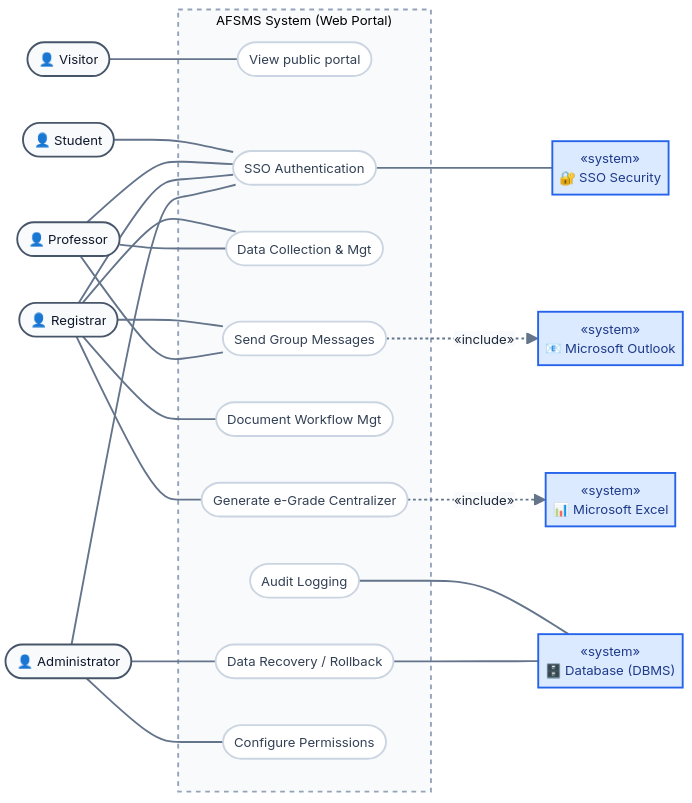
\includegraphics[width=0.85\textwidth]{1e.png}
      \vspace{0cm}
    }}
    \caption{System Use Case Diagram.}
    \label{fig:img1}
\end{figure}

\subsection{User Classes and Characteristics}
The AFSMS serves a diverse set of user classes, each with varying levels of technical expertise, frequency of use, and access privileges. The user classes are listed below in order of their importance to the system's core administrative success:

\begin{table}[H]
\centering
\small
\setlength{\arraystretch}{0.85}
\begin{tabularx}{\textwidth}{>{\raggedright\arraybackslash}p{2.2cm} >{\raggedright\arraybackslash}X >{\raggedright\arraybackslash}X >{\raggedright\arraybackslash}X}
\toprule
\textbf{User Class} & \textbf{Characteristics} & \textbf{Frequency} & \textbf{Impact on Requirements} \\
\midrule
Registrar/ Secretariat & Intermediate IT skills, proficient in Excel/Outlook. & Daily/continuous. & Error-proof interfaces, 3-min usability, Excel/Outlook integration. \\
\midrule
Professors/ Staff & Varying technical expertise. & Intermittent, peaks at exams. & Intuitive interfaces, zero retraining, SSO security. \\
\midrule
Students & High digital literacy, mobile users. & Frequent, academic year. & Read-only access, limited scope, responsive. \\
\midrule
System Admin & Advanced DB/technical skills. & Occasional maintenance. & Audit logs, permissions, rollback/recovery. \\
\midrule
Public/Visitors & Unknown backgrounds. & Occasional. & Public view, curricula/timetables visibility. \\
\midrule
QA/Testers & Validation experts. & Intensive pre-deployment. & Verifiable requirements, stress tests. \\
\bottomrule
\end{tabularx}
\normalsize
\setlength{\arraystretch}{1.3}
\end{table}

\subsection{Operating Environment}
The AFSMS operates in a client-server architecture and will function in the following specific environments:

\textbf{Server Environment (Backend and Database)}
\begin{itemize}
    \item \textbf{Hardware Platform:} Physical servers hosted within the university data center or virtualized infrastructure (cloud) equipped with scalable processing and storage resources required for large data volumes.
    \item \textbf{Operating Systems:} Compatibility with server-grade distributions such as Linux (e.g., Ubuntu Server 22.04 LTS, Ubuntu Server 24.04 LTS, CentOS) or Windows Server (2019, 2022).
    \item \textbf{Software Components:} A robust relational Database Management System (DBMS) that supports complex queries, offline backups, and rollback operations (point-in-time recovery).
\end{itemize}

\textbf{Client Environment (Frontend / User Interface)}
\begin{itemize}
    \item \textbf{Hardware Platform:} Any internet-connected device. The application will run smoothly on desktop PCs and laptops used in the registrar's office, as well as mobile-capable devices (e.g., modern sleek web tablets or smartphones).
    \item \textbf{Operating Systems:} Windows (10, 11), macOS, desktop Linux distributions, Android, iOS.
    \item \textbf{Web Browsers:} Access to the interface requires a modern, up-to-date browser (e.g., Google Chrome version 100+, Mozilla Firefox version 100+, Microsoft Edge, Apple Safari).
\end{itemize}

\textbf{Coexistence with Other Applications (Peaceful Coexistence)}
\begin{itemize}
    \item On user workstations (especially registrar office staff), the client component must coexist peacefully and functionally integrate with Microsoft Excel (versions 2016, 2019, 2021, or Microsoft 365) and Microsoft Outlook.
    \item The AFSMS system must allow these programs to run concurrently without memory conflicts, facilitating smooth document management, CSV/XLS file import/export, and seamless institutional communication.
\end{itemize}

\subsection{Design and Implementation Constraints}
The developers' choices regarding system architecture, UI design, and technologies are strictly limited by the following constraints:

\begin{itemize}
    \item \textbf{Regulatory and Corporate Policies:} The system must strictly comply with EU/Romanian GDPR regulations regarding personal student data handling, as well as the University of Craiova's internal corporate policies for academic data retention.
    \item \textbf{Hardware Limitations (Memory Requirements):} The server architecture is constrained by the need for expansive, scalable memory to support the permanent storage of comprehensive activity logs required for the point-in-time recovery feature.
    \item \textbf{Specific Technologies and Databases:} The backend must utilize a robust relational Database Management System (DBMS). The frontend must be developed using standard web technologies (HTML/CSS/JS) to ensure cross-platform compatibility without requiring local client installations.
    \item \textbf{Security Considerations and Communications Protocols:} All data transfers must occur over secure HTTPS protocols. Authentication should support integration with institutional security mechanisms (e.g., SSO if available).
    \item \textbf{Interfaces to Other Applications:} Export and communication modules are strictly constrained to interface natively with Microsoft Excel (.XLS/.CSV) and Microsoft Outlook.
    \item \textbf{Design Conventions and Programming Standards:} To ensure standardized data entry, developers are constrained to predominantly use selection lists (dropdowns) rather than free-text input fields. Report data must be displayed exclusively in tabular formats.
    \item \textbf{Audit, Control, and Parallel Operations (Criticality):} Managing critical academic records requires absolute data integrity. The DBMS must natively support full activity logging (audit) and point-in-time rollback capabilities (control). The system must safely handle heavy parallel operations (concurrent access) during peak exam sessions without signal timing failures or data corruption.
\end{itemize}

\subsection{User Documentation}
To ensure high adoption rates and reduce the learning curve across all user classes, a comprehensive suite of user documentation will be delivered alongside the AFSMS software. The documentation will be meticulously organized by user roles and will adhere strictly to modern technical writing standards.

\subsubsection{Delivered Documentation Components}
\begin{itemize}
    \item \textbf{Registrar \& Secretariat Staff Operations Manual:}
    \begin{itemize}
        \item \textit{Scope:} An exhaustive guide detailing daily workflows and data entry procedures.
        \item \textit{Contents:} Step-by-step instructions for data collection via dropdowns, managing electronic document circulation, and utilizing advanced search filters. Includes detailed chapters on native Excel integration for data export/import, triggering Outlook communications, and generating the e-Transcript (Registrul matricol) and the e-Grade Centralizer.
    \end{itemize}
    \item \textbf{Professors \& Teaching Staff Quick Start Guide:}
    \begin{itemize}
        \item \textit{Scope:} A concise, highly visual tutorial focused strictly on features relevant to faculty members.
        \item \textit{Contents:} Instructions for SSO authentication, locating study formations, inputting session grades, and finalizing evaluation records before deadlines.
    \end{itemize}
    \item \textbf{System \& Database Administrator Guide:}
    \begin{itemize}
        \item \textit{Scope:} Highly technical documentation for IT staff responsible for maintaining the system infrastructure.
        \item \textit{Contents:} Procedures for initial site adaptation (configuring curricula, grid values), mapping user access privileges, managing the DBMS, interpreting activity logs, performing offline backups, and executing point-in-time database recoveries (rollback function).
    \end{itemize}
    \item \textbf{Student Portal Guide (Online Help):}
    \begin{itemize}
        \item \textit{Scope:} A brief, accessible FAQ embedded directly into the private portal.
        \item \textit{Contents:} Instructions on how to view personal schedules, interpret grade records, and request official administrative documents.
    \end{itemize}
\end{itemize}

\subsubsection{Interactive and In-App Documentation}
\begin{itemize}
    \item \textbf{Context-Sensitive Help:} The web interface will feature embedded tooltips (hover-text) next to complex fields and dropdowns to assist users proactively without requiring external manuals.
    \item \textbf{Error Resolution Prompts:} Client-side validation errors will be accompanied by in-app text directly suggesting resolution methods (e.g., ``Invalid format: Please ensure the Excel file matches the provided .XLS template before importing'').
\end{itemize}

\subsubsection{Delivery Formats and Tooling}
The user documentation for AFSMS will be delivered in the following formats:
\begin{itemize}
    \item \textbf{Web-Based Documentation:} A structured online help section integrated within the web portal. This will provide easy access to user guides, FAQs, and contextual help directly from the application interface.
    \item \textbf{PDF Manuals:} Comprehensive user manuals (Registrar Guide, Professor Guide, Administrator Guide) will be delivered in PDF format for offline access, printing, and institutional archiving purposes.
\end{itemize}
All documentation will be written in clear, structured language and updated alongside major software releases to reflect system changes and improvements.

\subsubsection{Documentation Standards and Compliance}
The creation and formatting of all user documentation will strictly adhere to the following standards:
\begin{itemize}
    \item \textbf{ISO/IEC/IEEE 26514:2022:} Standard for the design and development of information for users of software (ensuring proper structure, task-oriented writing, and clarity).
    \item \textbf{WCAG 2.2 (Level AA):} All HTML5-based documentation and PDF materials will comply with accessibility requirements to ensure usability for individuals with disabilities, including screen reader compatibility, sufficient color contrast, keyboard navigation, and accessible formatting.
    \item \textbf{GDPR Compliance in Documentation:} All sample data, screenshots, and tutorials within the documentation must use anonymized, synthetic ``dummy'' data to ensure no real student Personally Identifiable Information (PII) is exposed during training.
\end{itemize}

\subsection{Assumptions and Dependencies}
The requirements established within this SRS are heavily influenced by the following assumed factors and external dependencies. These factors are not inherently design constraints; rather, if any of these conditions are proven false or altered during the project lifecycle, the requirements stated in the SRS will need to be revised accordingly.

\subsubsection{Assumptions (Factors Assumed to be True)}
\begin{itemize}
    \item \textbf{A. Infrastructure and Provisioning:} It is assumed that the University of Craiova's IT department will provide an internal data center or cloud-hosting environment guaranteeing a baseline adequate availability during academic periods and sufficient bandwidth for concurrent exam-season traffic.
    \textit{Impact if false:} The SRS must be rewritten to include architectural requirements for a fully distributed, highly available external cloud architecture (e.g., AWS/Azure) and load-balancing protocols.
    \item \textbf{B. Centralized SSO Availability:} It is assumed that the university’s centralized Single Sign-On (SSO) security subsystem will provide a stable, standard authentication protocol endpoint (e.g., SAML 2.0 or OAuth 2.0) for seamless integration.
    \textit{Impact if false:} The design constraint prohibiting a standalone credential database (Section 2.5) must be invalidated. The SRS will require immediate addition of complex functional requirements for secure password hashing, credential storage, account recovery, and multi-factor authentication (MFA).
    \item \textbf{C. Browser Standards and Connectivity:} It is assumed that all end-users possess devices with reliable internet access capable of rendering modern web standards (HTML5, ES6 JavaScript). This applies equally to legacy desktop PCs in the secretariat and modern mobile hardware (e.g., smartphones, or tablets).
    \textit{Impact if false:} If specific network zones within the faculty lack reliable internet, or if users are constrained to deprecated browsers (e.g., Internet Explorer 11), the SRS must be updated to include requirements for an ``offline synchronization mode'' and polyfill support for legacy rendering engines.
    \item \textbf{D. Open-Source / Commercial Libraries:} It is assumed that the development team will have unrestricted access to necessary open-source or commercial software libraries required for generating standard export formats (CSV, XML, XLS, PDF) without facing institutional licensing blockades.
    \textit{Impact if false:} The functional requirements mandating specific export formats will need to be scoped down to simple text exports, or the project budget/timeline must be explicitly expanded in the project plan.
    \item \textbf{E. Administrative User Training:} It is assumed that registrar and secretariat staff will undergo a mandatory minimum 1-hour training session prior to system deployment.
    \textit{Impact if false:} The verifiable performance requirement (generating an e-Centralizer in under 3 minutes) cannot be fairly evaluated during User Acceptance Testing (UAT) and must be removed from the SRS.
\end{itemize}

\subsubsection{Dependencies (External Factors Relied Upon)}
\begin{itemize}
    \item \textbf{A. Microsoft Office Ecosystem:} The system's automated data export, import, and communications modules are wholly dependent on the continued availability, licensing, and file-format stability of Microsoft Excel and Microsoft Outlook on the registrar staff's local machines. If Microsoft drastically deprecates local interoperability protocols or alters legacy .XLS parsing rules, the system's integration modules will require immediate refactoring.
    \item \textbf{B. Legacy Data Availability (Site Adaptation):} The operational launch of AFSMS is strictly dependent on the faculty secretariat providing cleansed, structured legacy data (historical student records, active curricula, past evaluation grid values) for the database seeding phase. Delays, omissions, or severe formatting errors in this source data will block the initial site adaptation and directly delay the software's deployment.
    \item \textbf{C. Regulatory Environment:} The system's activity logging, data retention, and point-in-time rollback features are legally dependent on the current state of EU/Romanian GDPR legislation and the Romanian Ministry of Education's data archiving mandates. Any future legislative amendments altering how long academic data must be retained or when it must be demonstrably destroyed will force mandatory revisions to the database architecture and automated pruning requirements.
    \item \textbf{D. Institutional Network Security Configurations:} The software's ability to send automated notifications and authenticate users is dependent on the university's central IT department configuring the institutional firewalls to whitelist the application's servers for outbound SMTP email traffic and inbound SSO callback requests.
\end{itemize}


% --- SECTION 3: EXTERNAL INTERFACE REQUIREMENTS ---
\section{External Interface Requirements}

\subsection{User Interfaces}
The AFSMS provides a web-based graphical user interface, accessible through modern browsers, and is organized into two main perspectives: a Public Portal (unauthenticated, read-only) and a Private Portal (authenticated via university SSO with role-based access control for registrar staff, professors, students, and system administrators).

\subsubsection{Logical Characteristics and Screen Organization}
\begin{itemize}
    \item \textbf{Window and Page Layouts:} The interface utilizes a persistent two-pane window organization. The left pane contains a fixed, role-based navigation sidebar. The main right pane serves as the dynamic workspace. Breadcrumb navigation is persistently displayed at the top of the workspace to prevent user disorientation.
    \item \textbf{Screen Formats:} All academic records (e.g., grade registers, centralizers) must be presented in a standard tabular format mirroring MS Excel to ensure familiarity for teaching and secretariat staff.
    \item \textbf{Standardized UI Elements:} Every authenticated screen must feature a persistent top header containing a universal search bar, user profile/logout controls, and a standardized ``Help'' icon that triggers context-sensitive assistance.
    \item \textbf{Keyboard Shortcuts:} The system shall support standard grid-navigation shortcuts (e.g., Tab to cycle through grade input columns, Enter to save the current row and advance) to optimize repetitive data entry.
\end{itemize}

\subsubsection{UI Optimization and Verifiable Usability}
\begin{itemize}
    \item \textbf{The ``Selection-Only'' Mandate (Do's and Don'ts):} To dramatically minimize data entry errors, the UI must utilize searchable dropdown menus (e.g., Select2/React-Select) for all relational data inputs (e.g., selecting study formations, subjects, or academic years). The UI must not use free-text input fields unless strictly required for non-standardized descriptions.
    \item \textbf{Error Message Standards:} The system shall display brief, non-technical error notifications immediately adjacent to the offending input field (e.g., ``Grade must be an integer between 1 and 10''). A ``More Info'' toggle must be provided on system-level errors to display long-form, technical descriptions for IT troubleshooting.
    \item \textbf{Verifiable Usability Requirement:} A secretariat staff member can successfully compile and export a complete semester e-Grade Centralizer for a study group of 30 students in under 3 minutes, after receiving no more than 1 hour of basic system training.
\end{itemize}

\begin{figure}[htbp]
    \centering
    \begin{minipage}{0.49\textwidth}
        \centering
        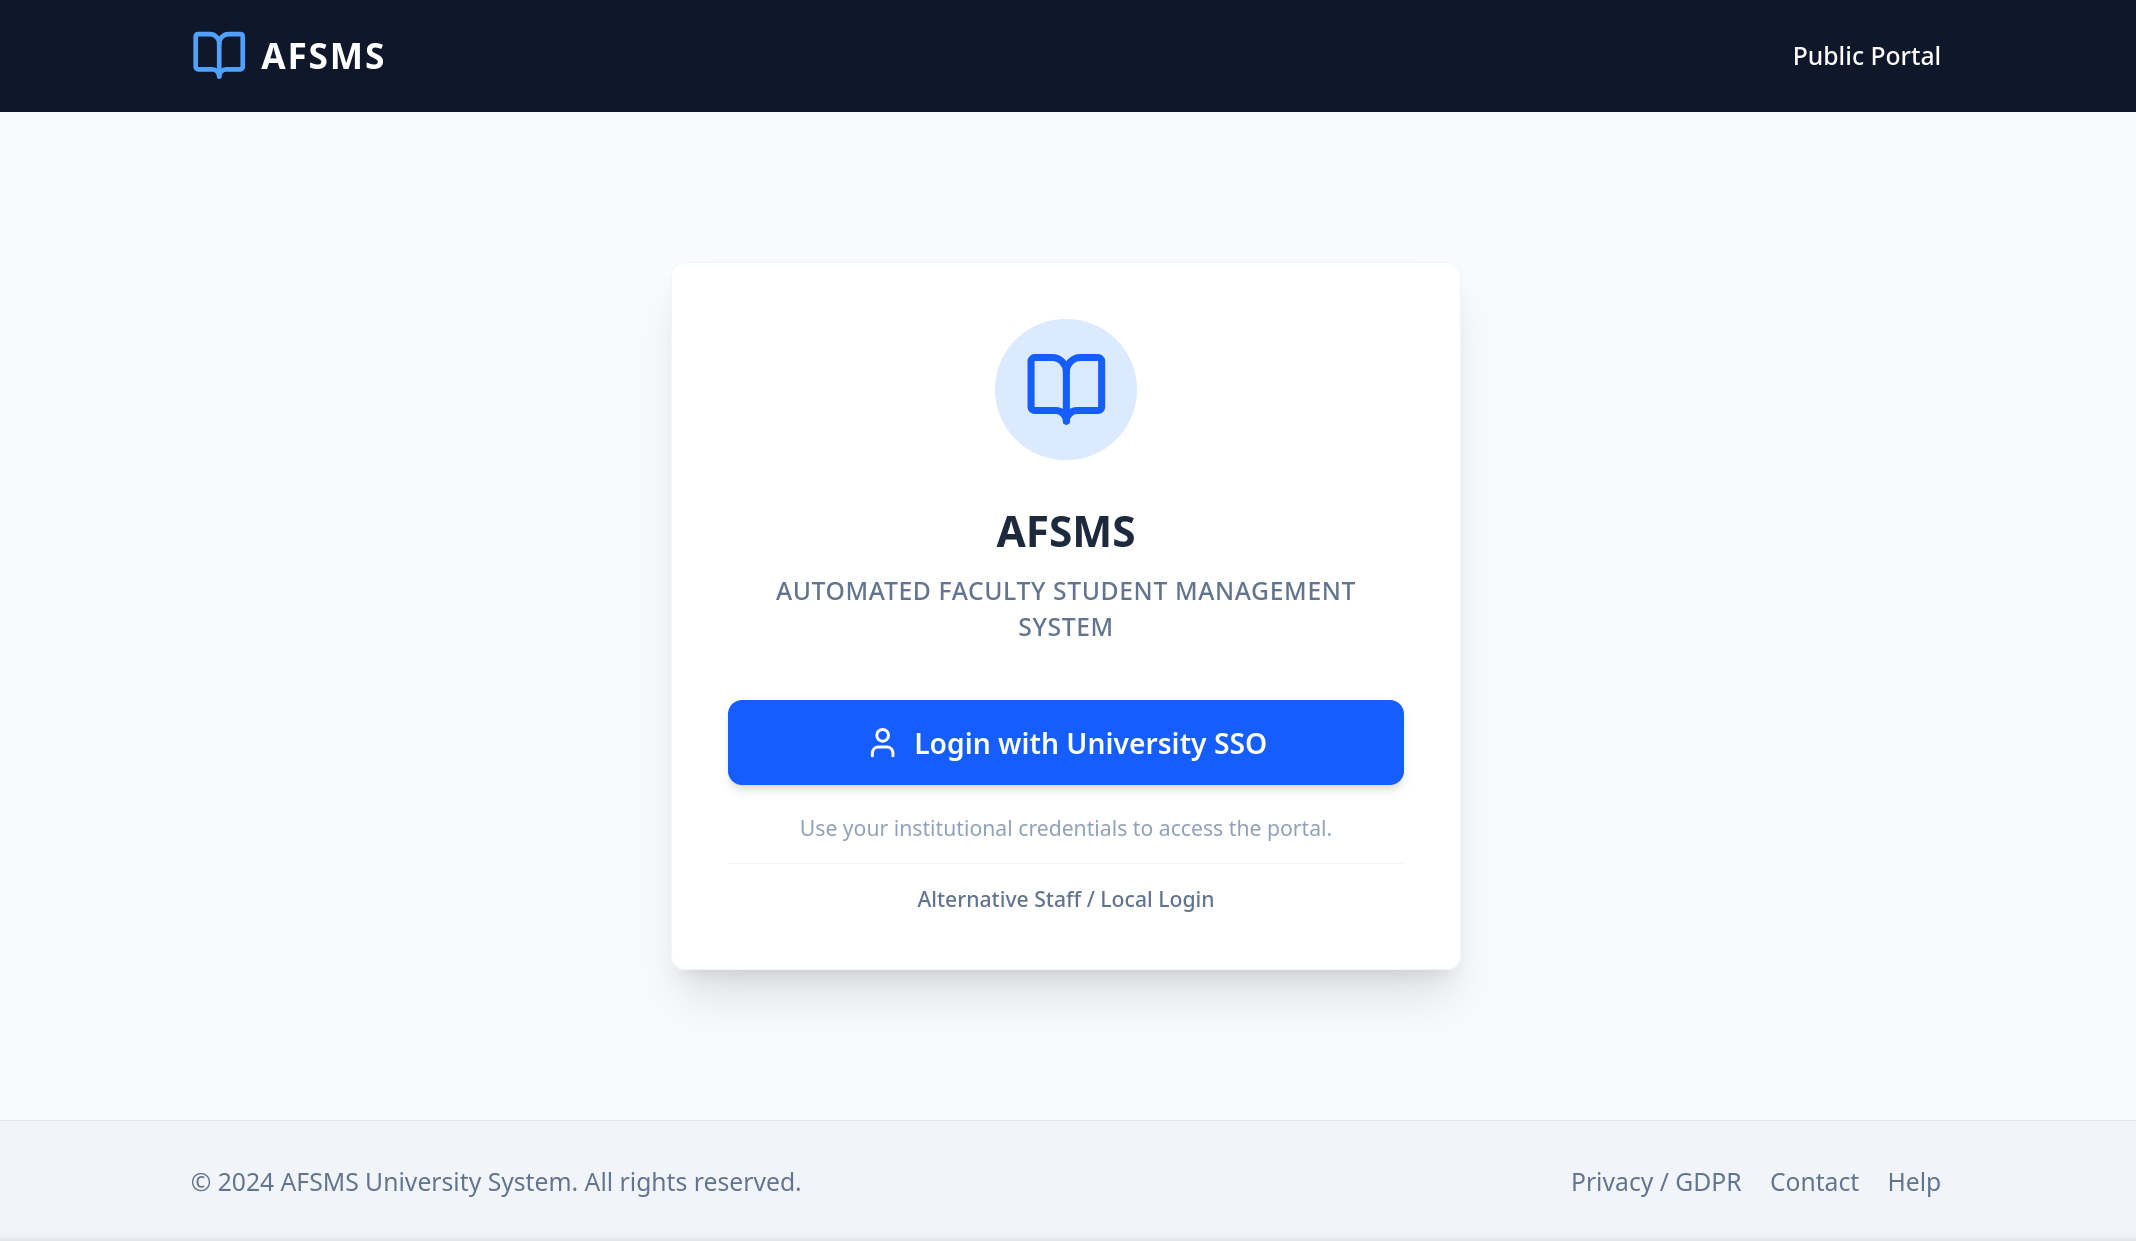
\includegraphics[width=\textwidth]{6.png}
        \caption{Students \& Curricula Management UI.}
        \label{fig:img6}
    \end{minipage}
    \hfill
    \begin{minipage}{0.49\textwidth}
        \centering
        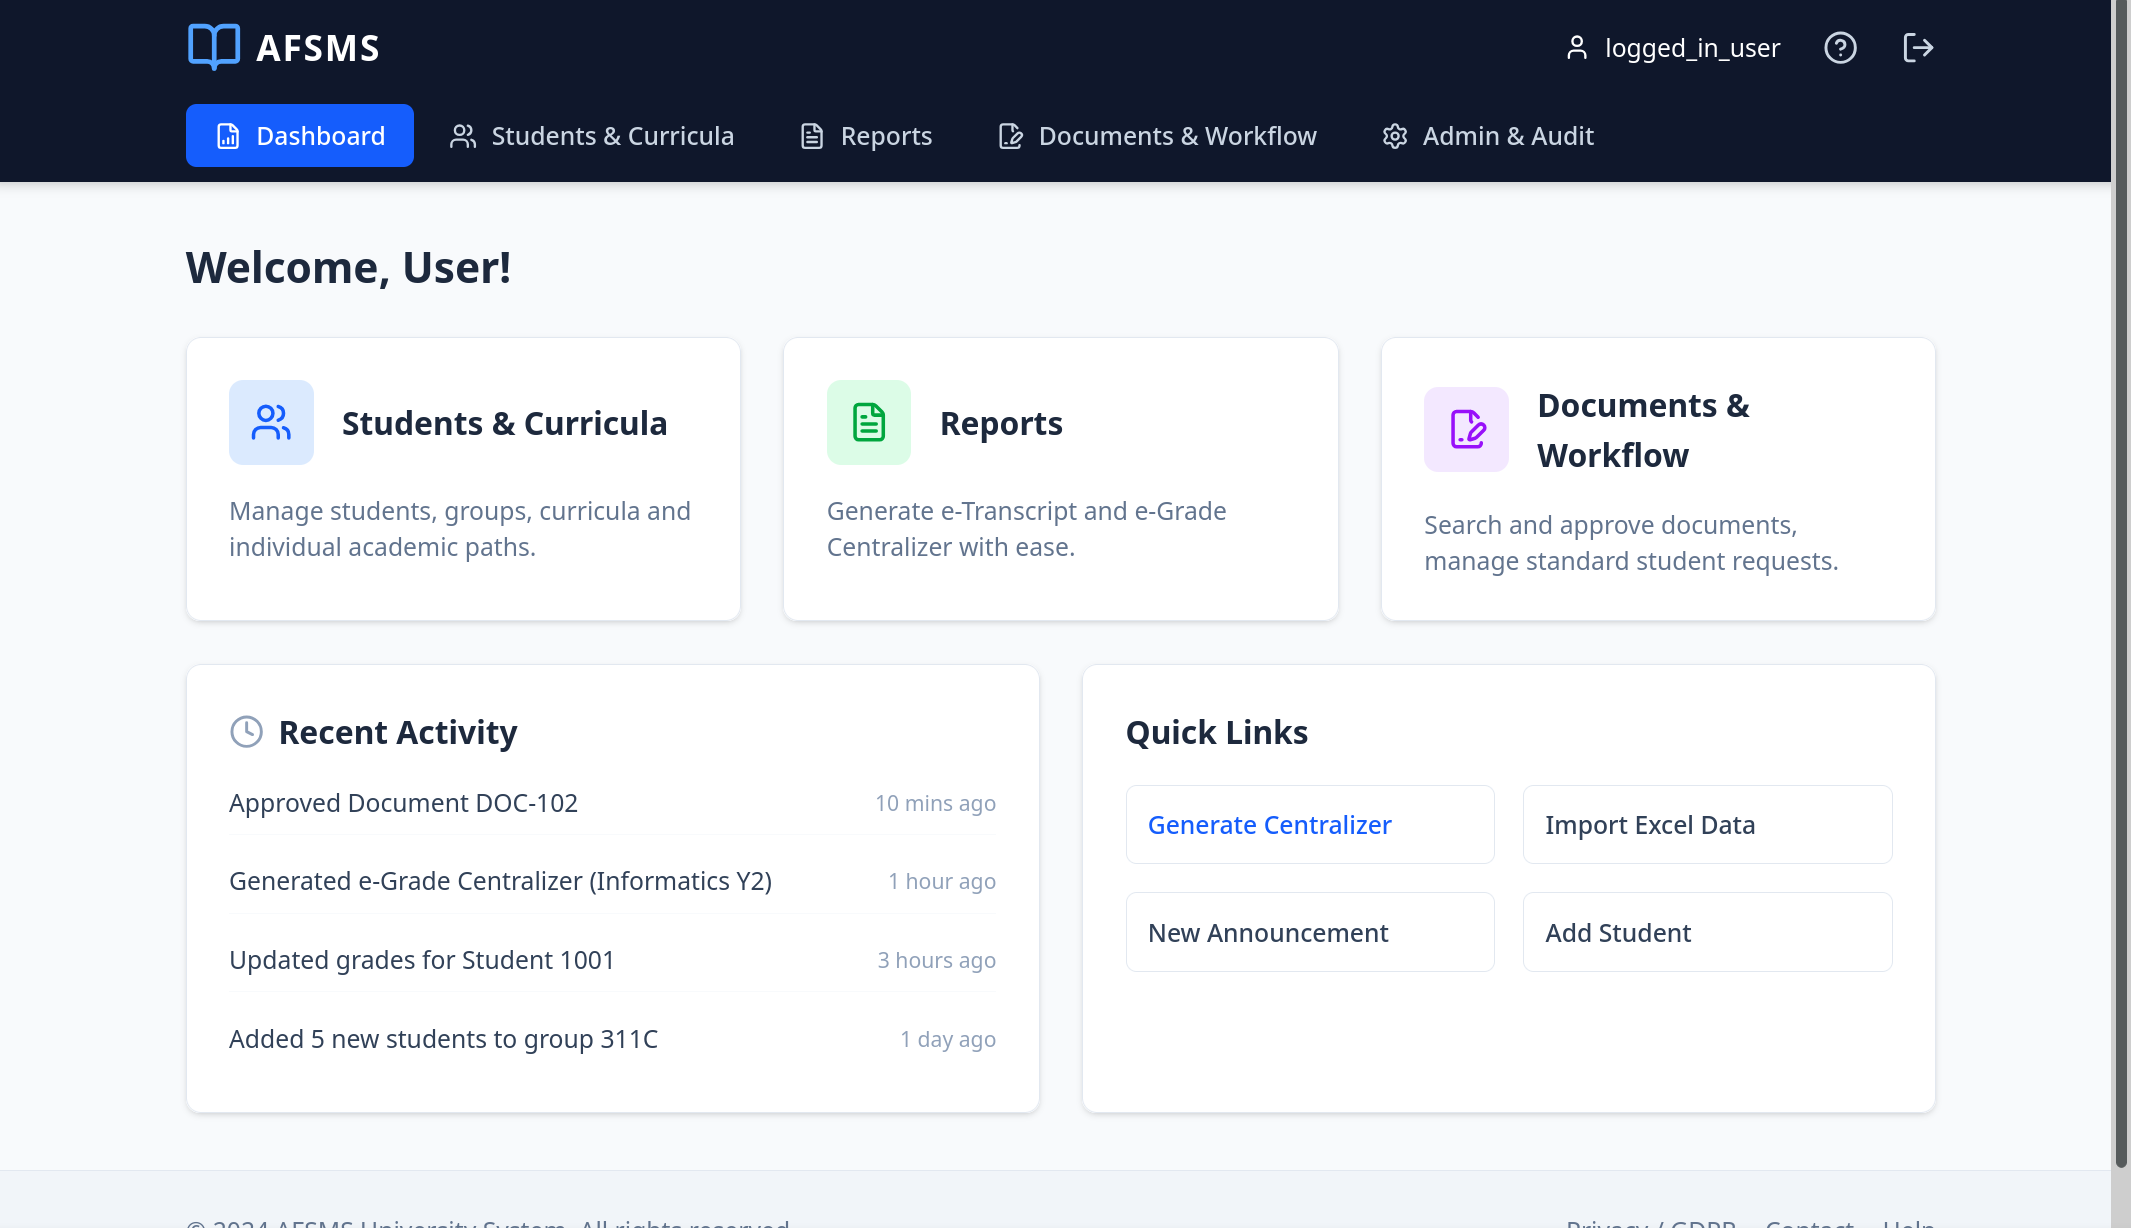
\includegraphics[width=\textwidth]{7.png}
        \caption{Data Collection Flowchart.}
        \label{fig:img7}
    \end{minipage}
\end{figure}

\begin{figure}[htbp]
    \centering
    \begin{minipage}{0.49\textwidth}
        \centering
        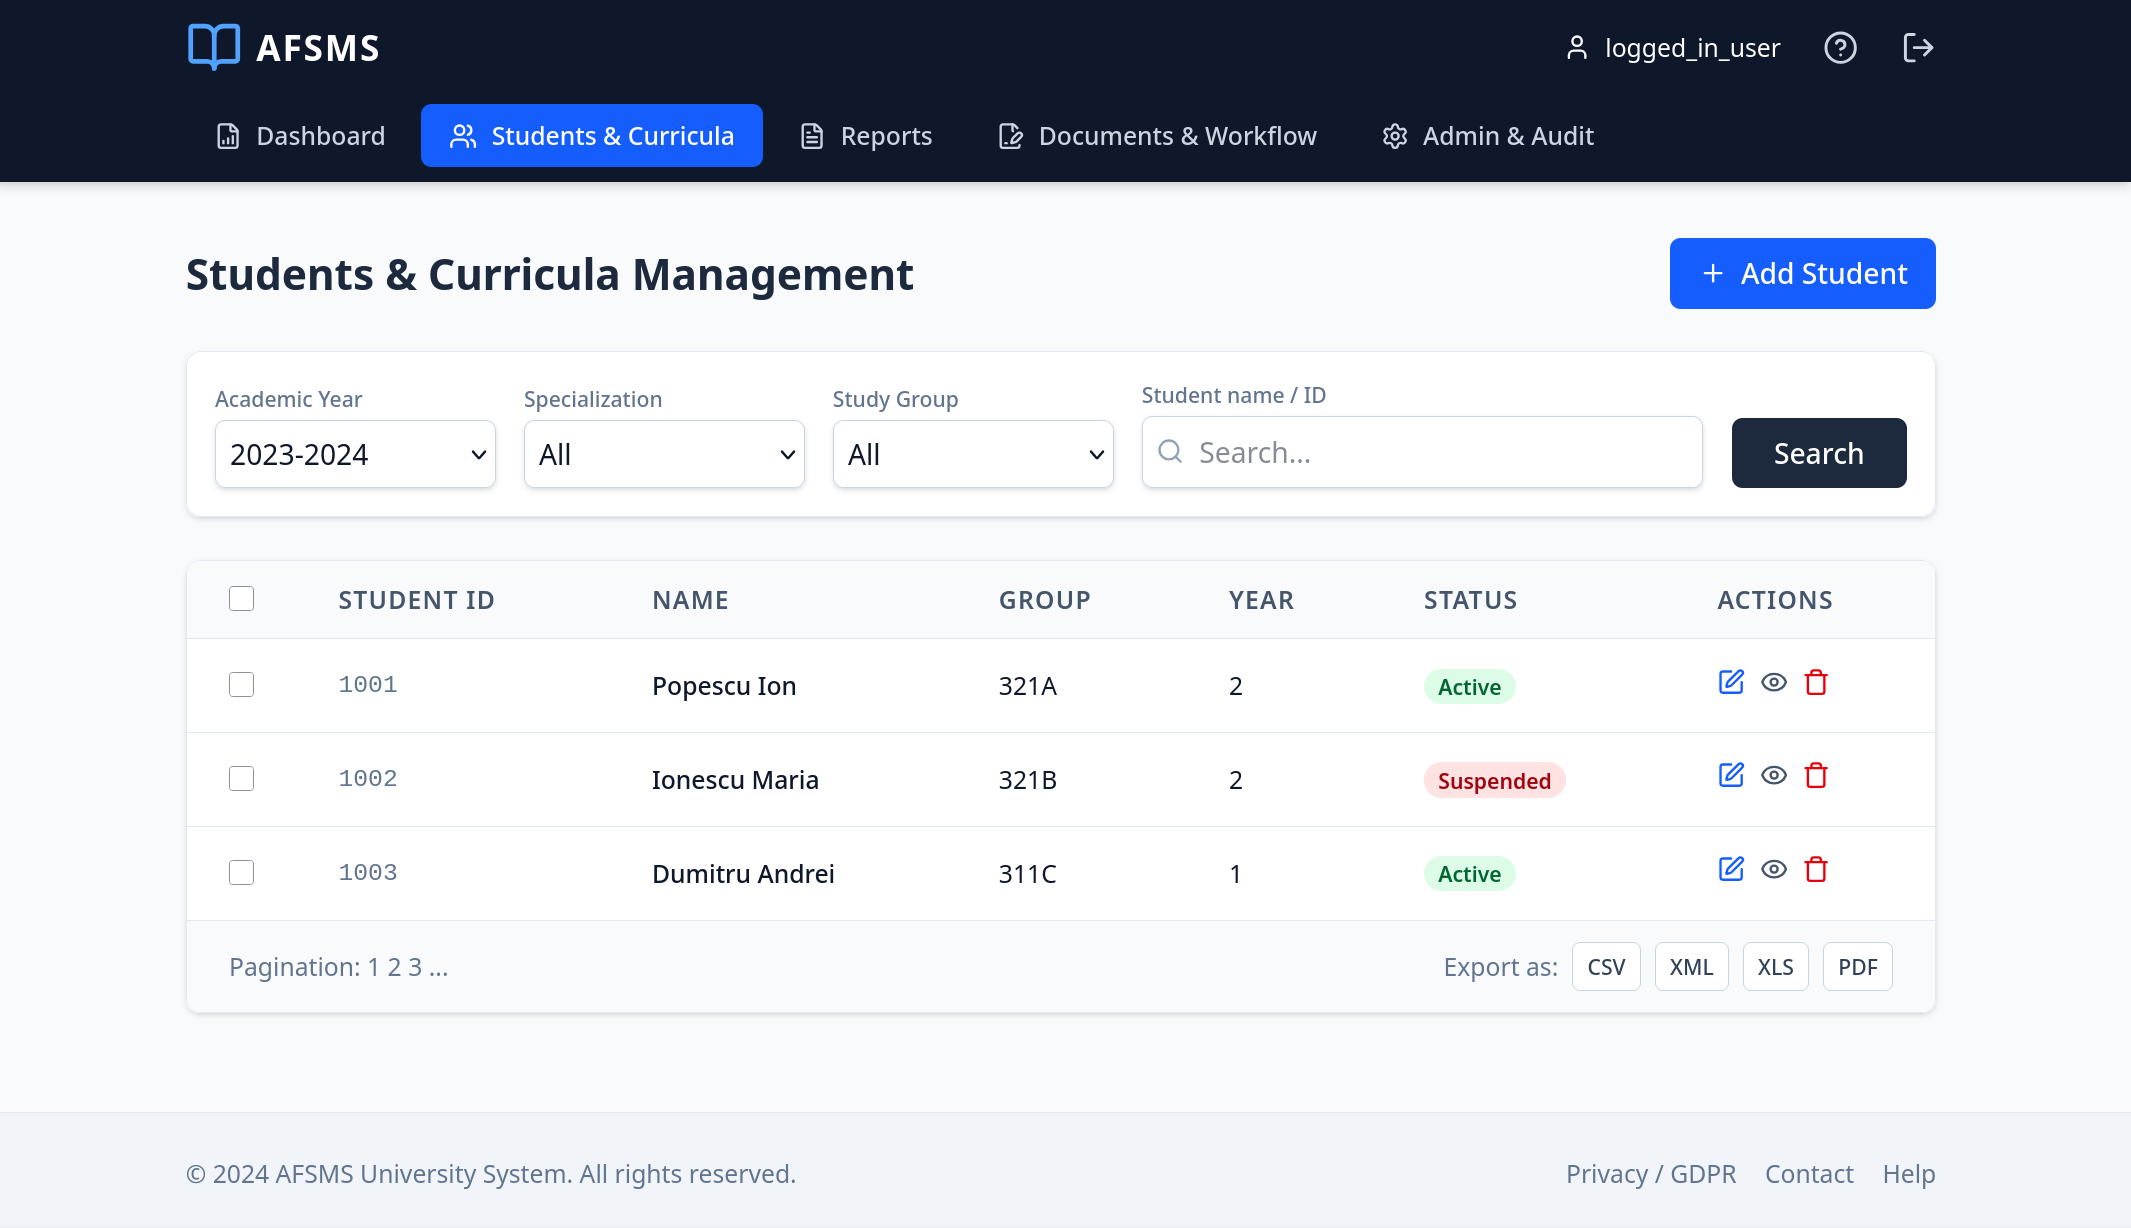
\includegraphics[width=\textwidth]{8.png}
        \caption{Reports - e-Grade Centralizer UI.}
        \label{fig:img8}
    \end{minipage}
    \hfill
    \begin{minipage}{0.49\textwidth}
        \centering
        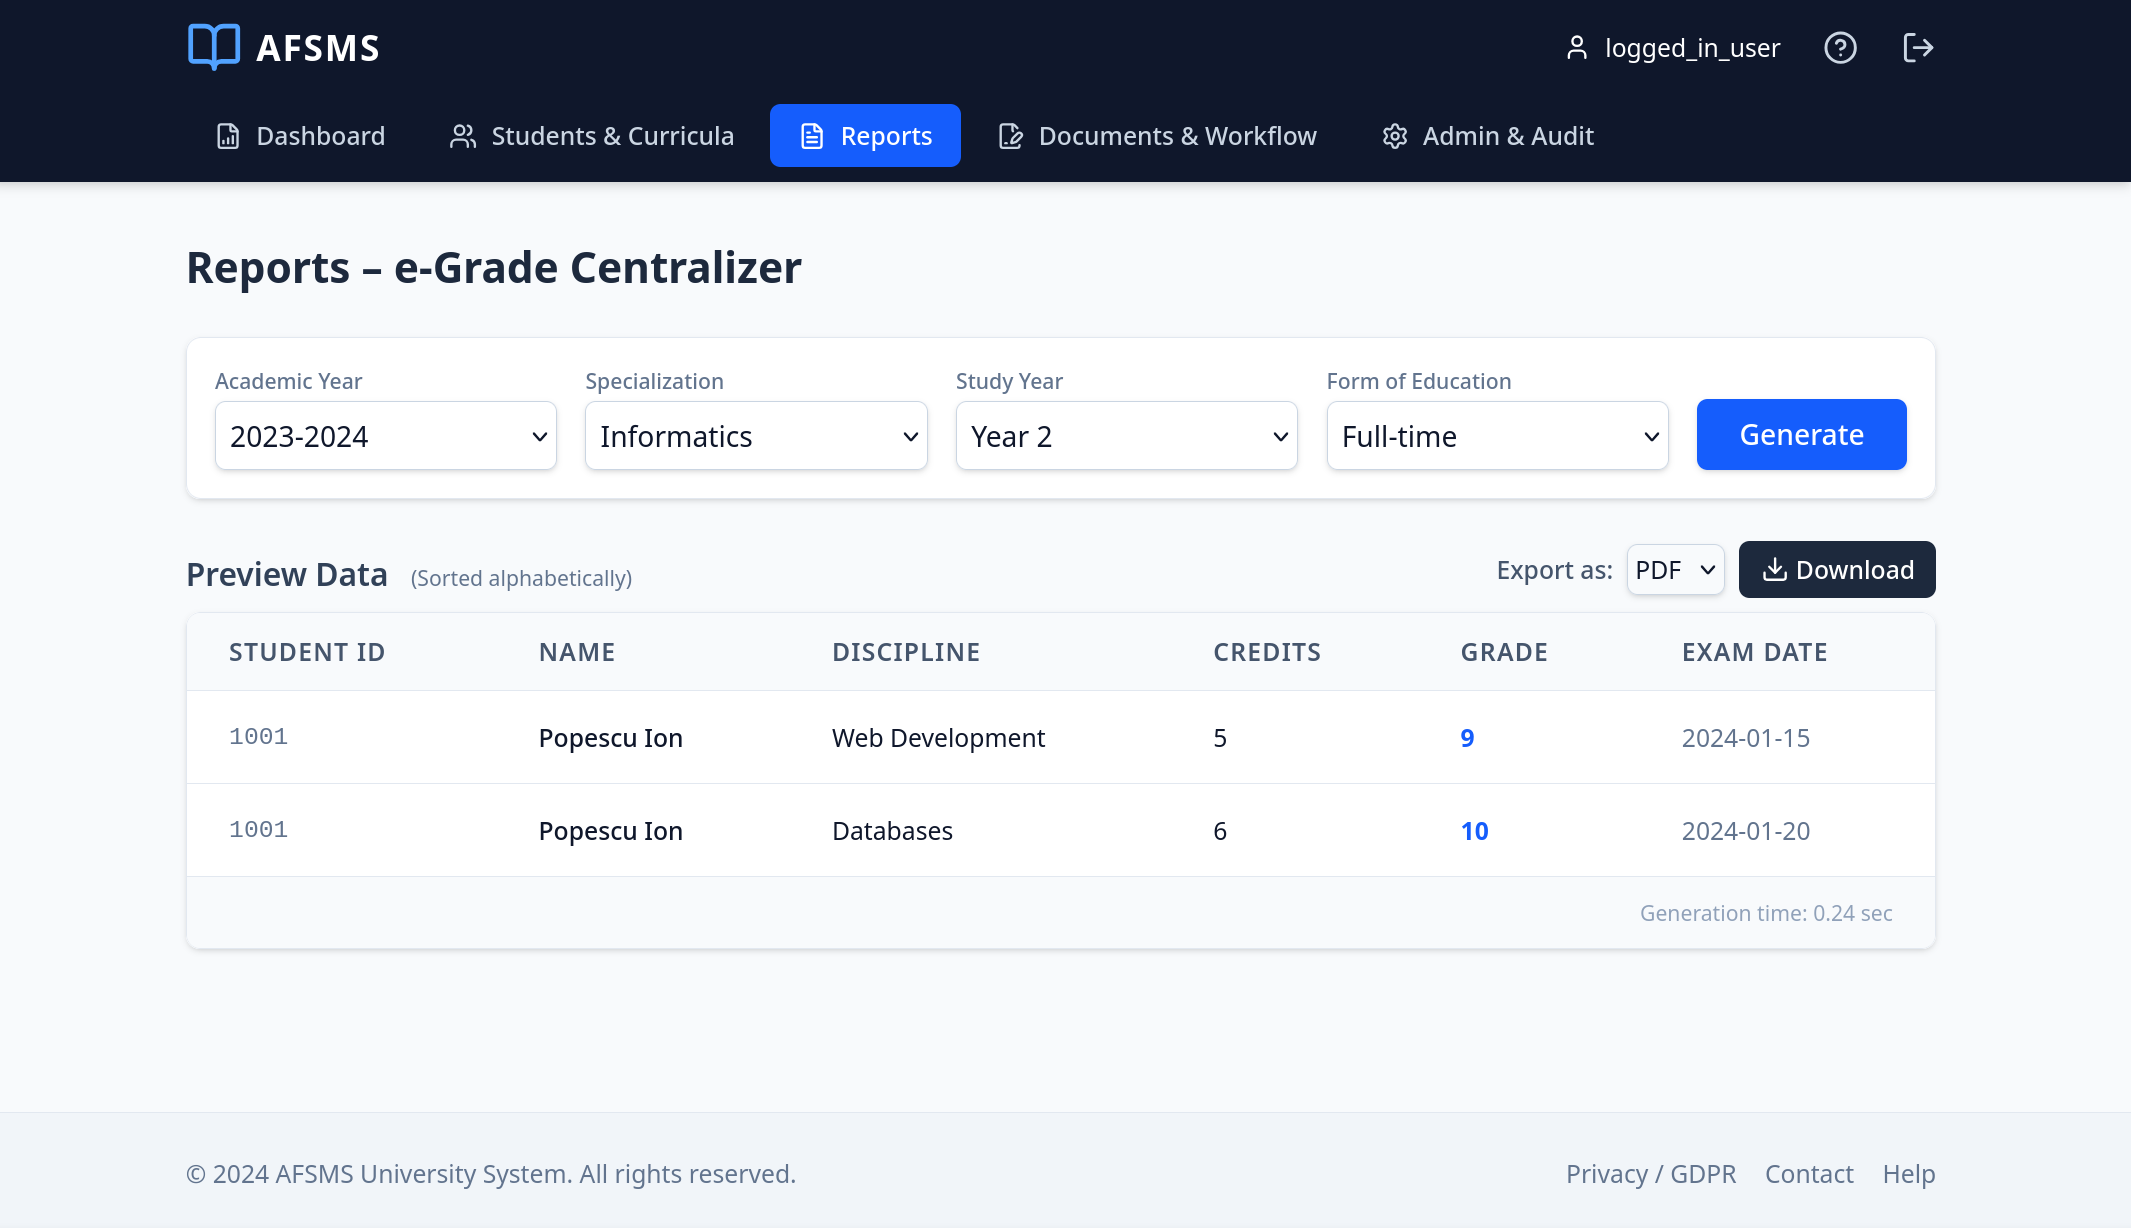
\includegraphics[width=\textwidth]{9.png}
        \caption{Documents \& Workflow UI.}
        \label{fig:img9}
    \end{minipage}
\end{figure}

\begin{figure}[htbp]
    \centering
    \begin{minipage}{0.49\textwidth}
        \centering
        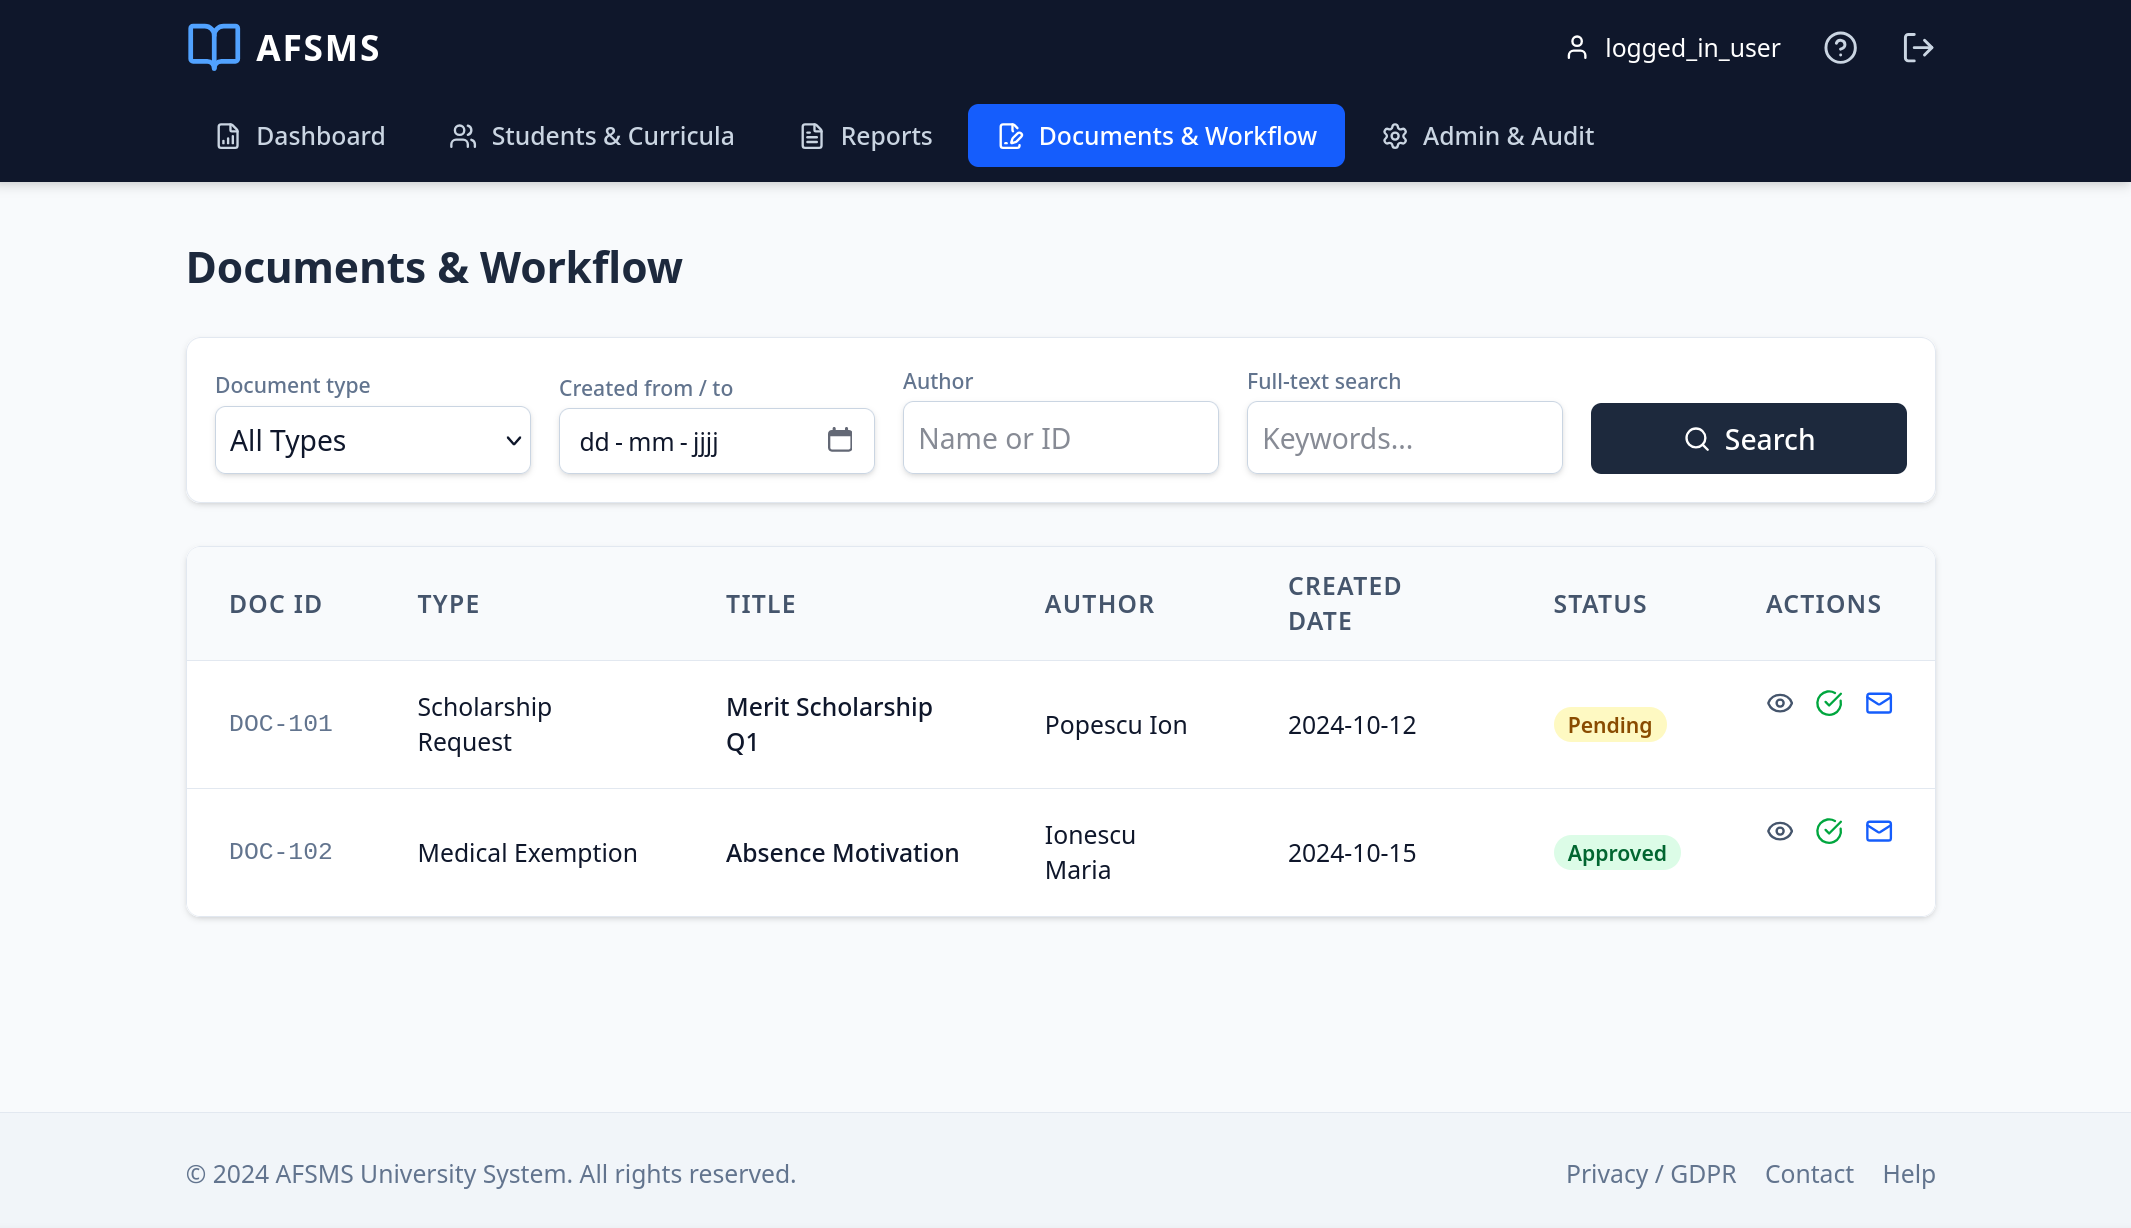
\includegraphics[width=\textwidth]{10.png}
        \caption{User Groups \& Messaging.}
        \label{fig:img10}
    \end{minipage}
    \hfill
    \begin{minipage}{0.49\textwidth}
        \centering
        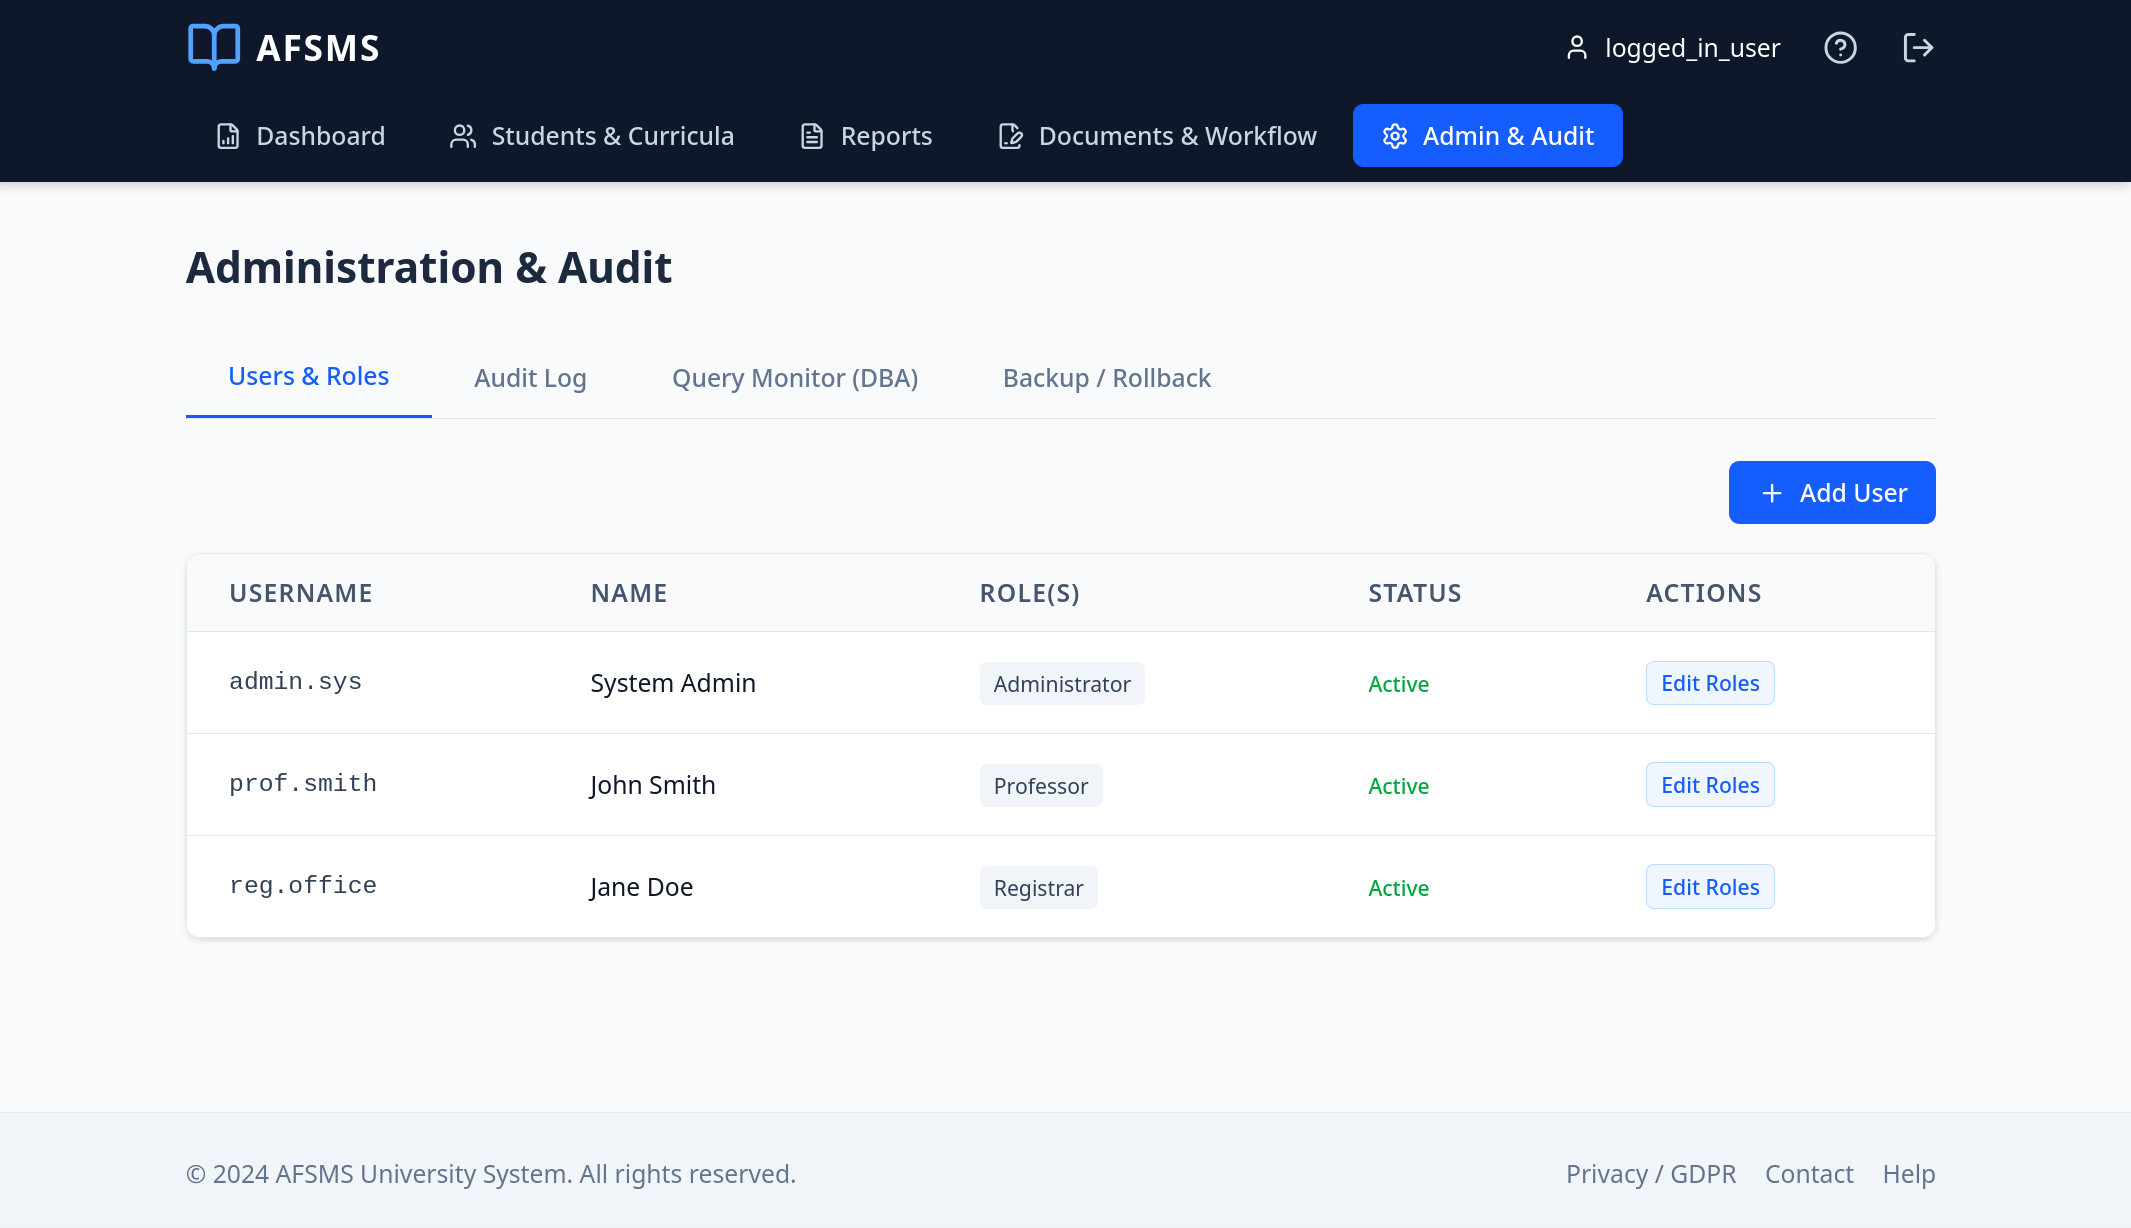
\includegraphics[width=\textwidth]{11.png}
        \caption{Administration \& Audit - Users \& Roles.}
        \label{fig:img11}
    \end{minipage}
\end{figure}

\begin{figure}[htbp]
    \centering
    \begin{minipage}{0.49\textwidth}
        \centering
        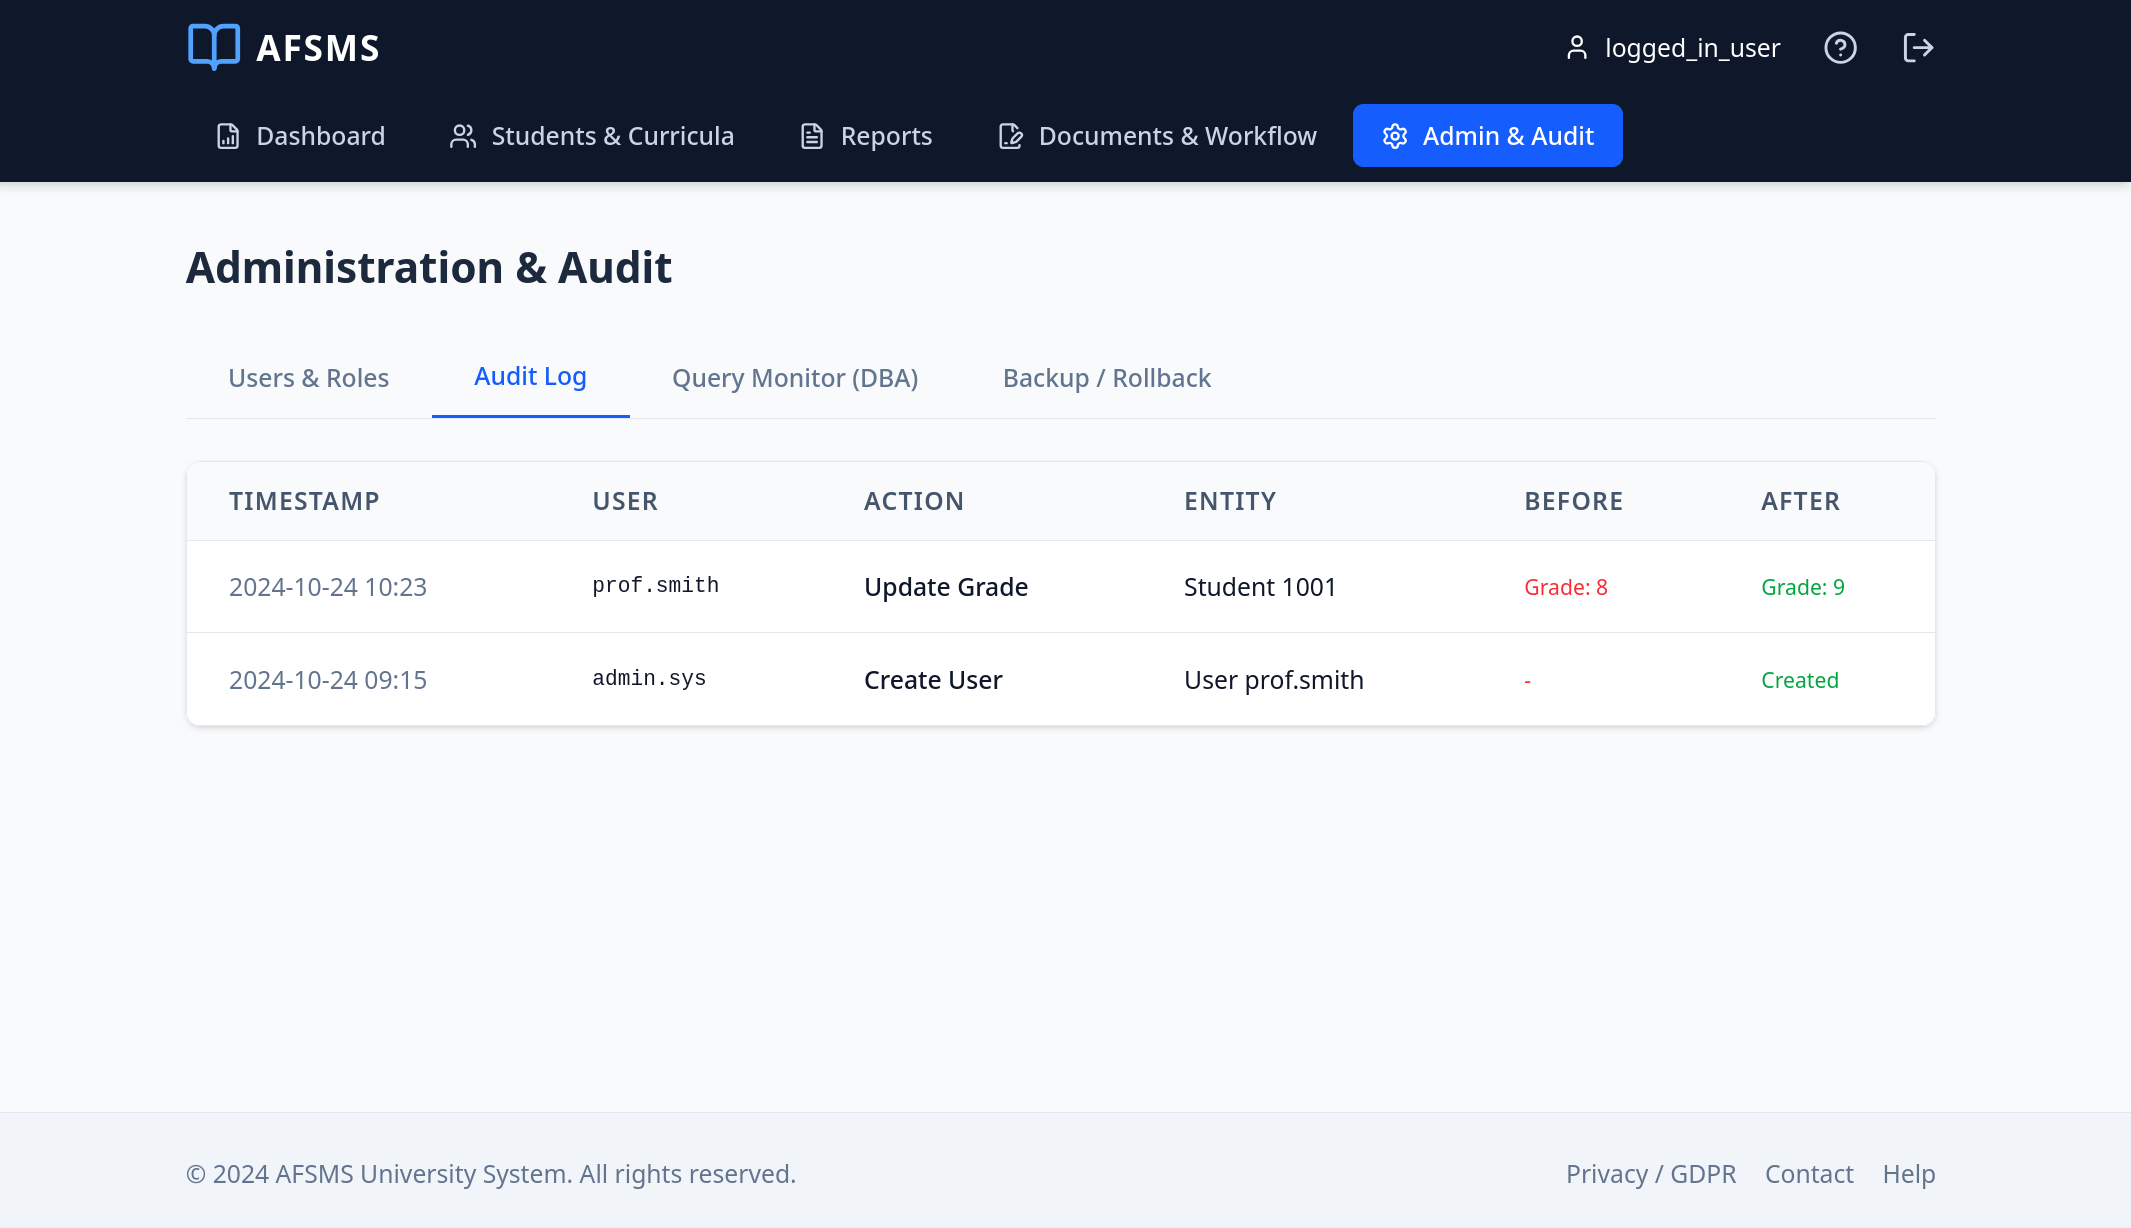
\includegraphics[width=\textwidth]{12.png}
        \caption{Administration \& Audit - Audit Log.}
        \label{fig:img12}
    \end{minipage}
    \hfill
    \begin{minipage}{0.49\textwidth}
        \centering
        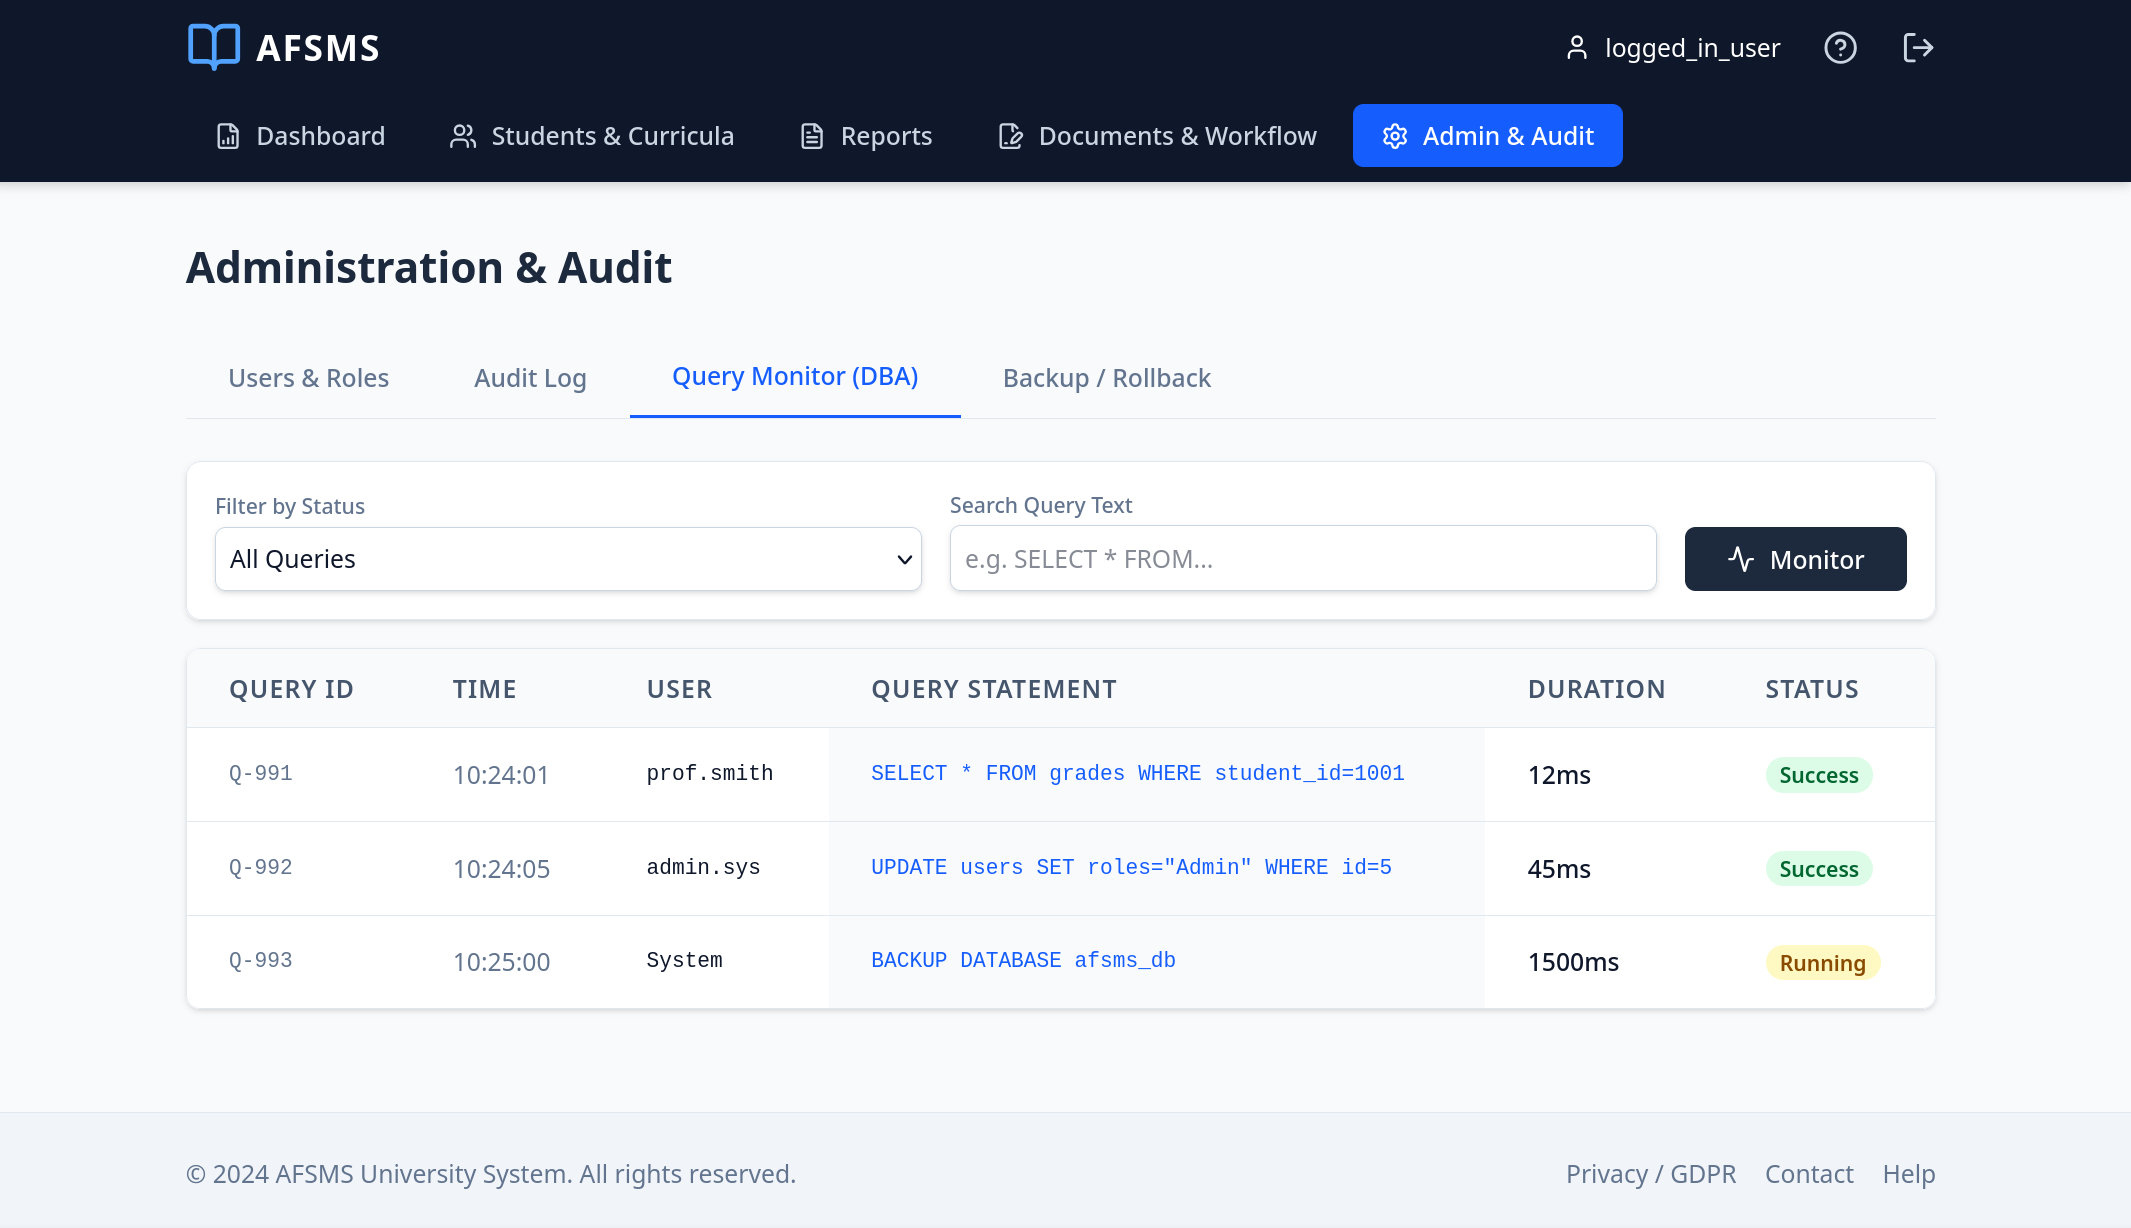
\includegraphics[width=\textwidth]{13.png}
        \caption{Administration \& Audit - Backup / Rollback.}
        \label{fig:img13}
    \end{minipage}
\end{figure}

\begin{figure}[htbp]
    \centering
    \begin{minipage}{0.49\textwidth}
        \centering
        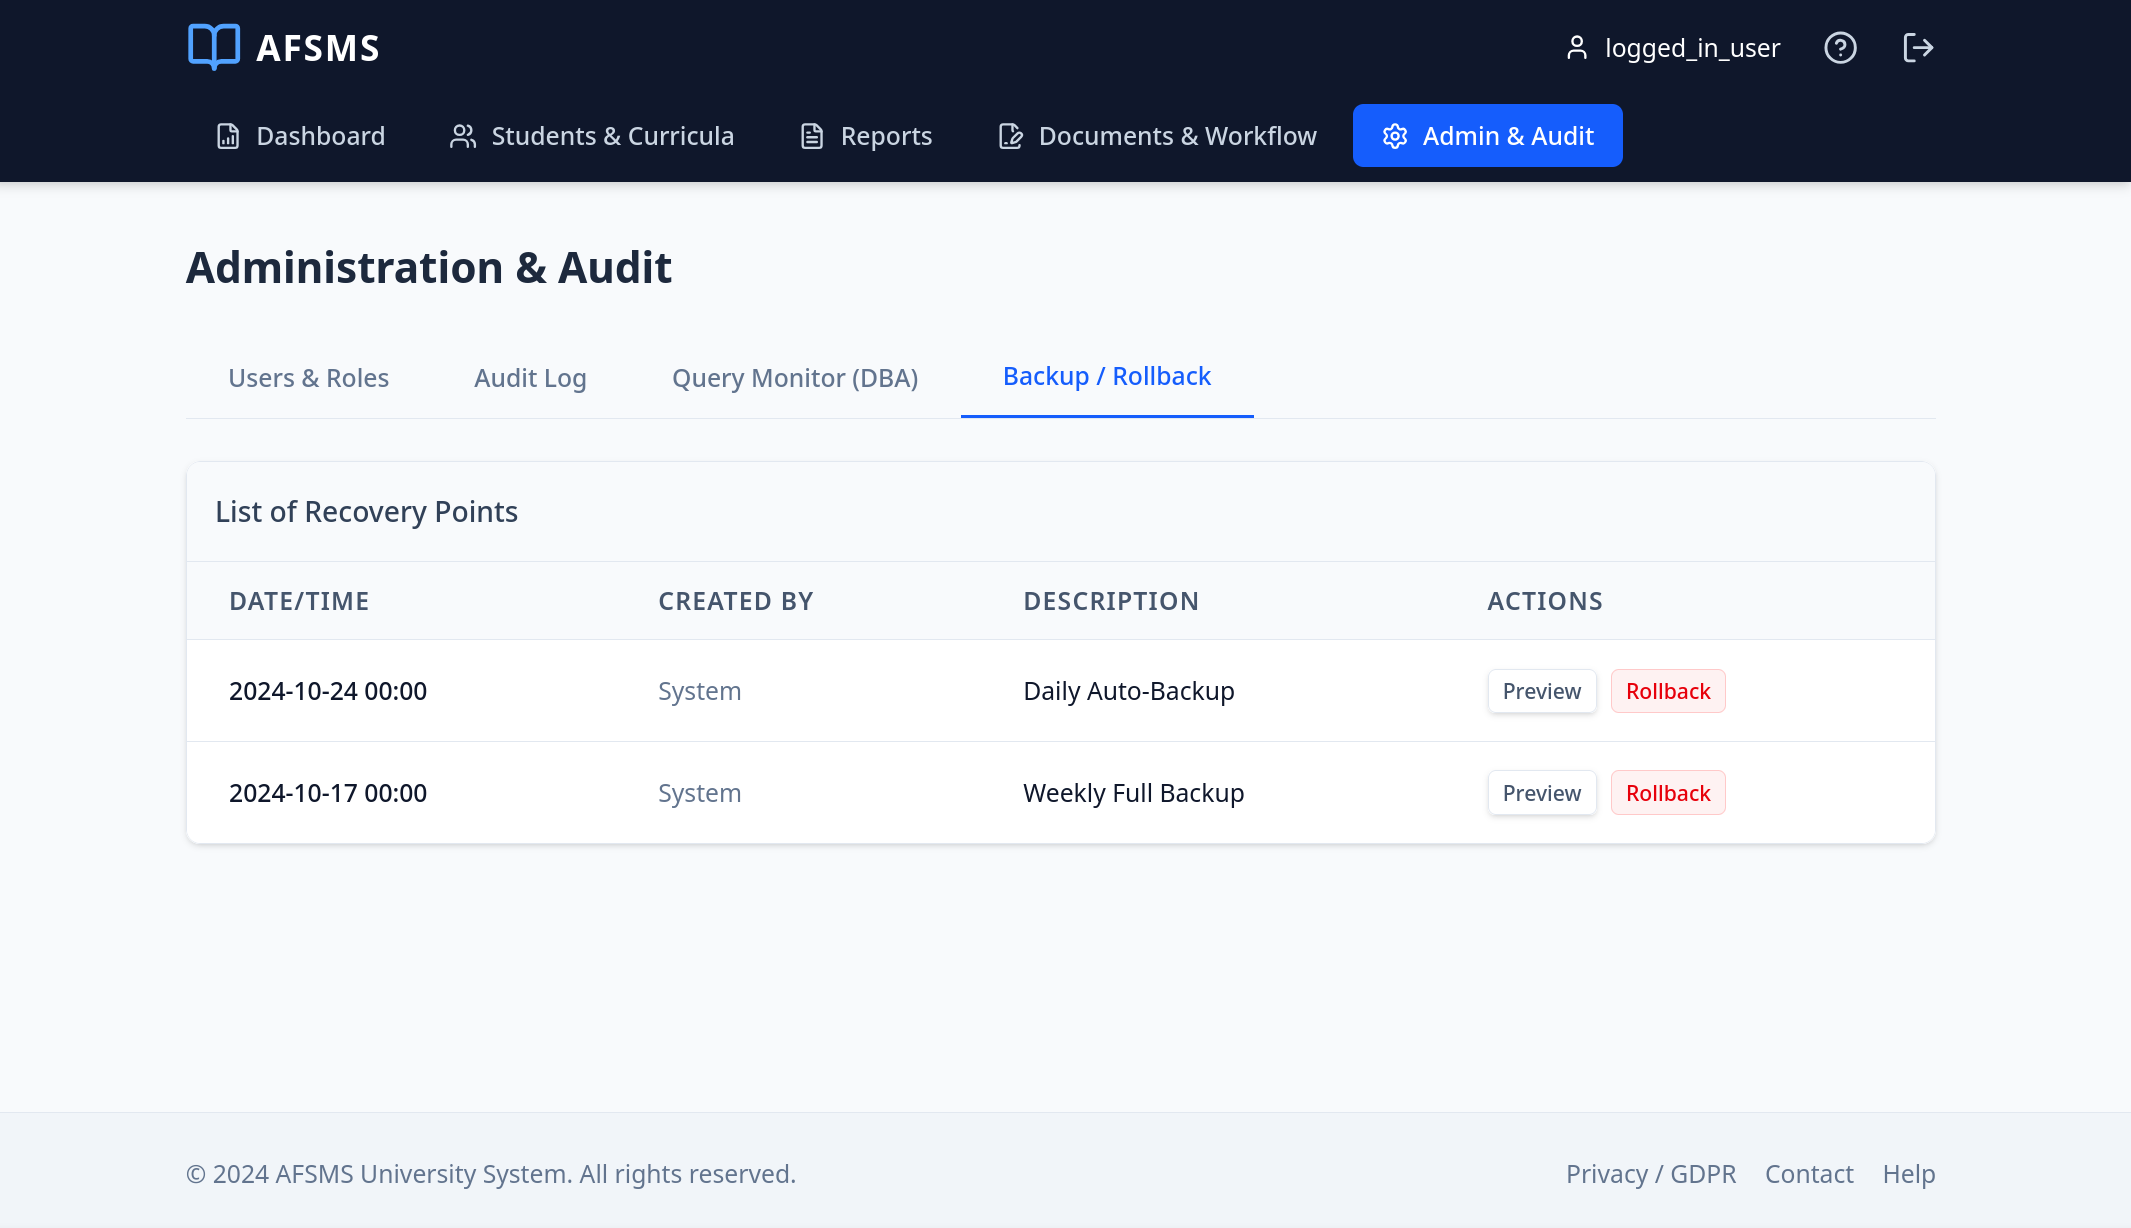
\includegraphics[width=\textwidth]{14.png}
        \caption{Rollback Point-in-Time Sequence Diagram.}
        \label{fig:img14}
    \end{minipage}
\end{figure}


\subsection{Hardware Interfaces}
AFSMS is a browser-based, client-server system; therefore, its hardware interfaces are defined primarily by the server infrastructure hosting the application and the end-user devices accessing the web portal. This section specifies the logical and physical characteristics of those interfaces in accordance with IEEE 5.2.1.3 and IEEE 5.3.1.

\subsubsection{Server-Side Hardware Interface}
\begin{itemize}
    \item \textbf{Deployment:} The system shall be deployable on either physical servers (on-premises) or virtualized infrastructure, provided the hardware supports multi-threaded concurrent processing.
    \item \textbf{Storage Interface:} The server hardware shall provide highly scalable primary and secondary storage to support a large operational database and the long-term retention of massive activity logs required for auditing and point-in-time recovery.
    \item \textbf{Network Interface:} The server shall expose the web application to client devices over standard network interfaces (Ethernet/Wi-Fi uplink via the institutional network).
\end{itemize}

\subsubsection{Client-Side Hardware Interface}
\begin{itemize}
    \item \textbf{Supported Devices:} The system shall be accessible from any internet-connected device capable of running a modern web browser, specifically including registrar office desktop PCs, laptops, modern web tablets, and smartphones.
    \item \textbf{Interaction Paradigm:} The interface shall provide full-screen graphical support within the browser, replacing any legacy line-by-line terminal interactions.
    \item \textbf{Peripherals:} The client side shall not require specialized hardware devices (e.g., barcode scanners, smart-card readers). The UI must support standard human input devices: keyboard and mouse on PCs/laptops, and touch input on mobile-capable devices.
\end{itemize}

\subsubsection{Hardware-Related Configuration Characteristics}
\begin{itemize}
    \item \textbf{Ports:} The system requires inbound TCP port 443 (HTTPS) to the web server hardware. Any other service ports (e.g., database administration) shall be physically or logically restricted to internal network interfaces.
    \item \textbf{Instruction Sets:} The client interface shall not depend on a specific CPU instruction set (e.g., x86 vs. ARM) or hardware architecture, as all hardware-level execution is abstracted by the standards-compliant web browser.
\end{itemize}

\subsubsection{Logical Characteristics of Hardware Interactions}
Because AFSMS is a web application, the following parameters apply strictly to the hardware-network layer and physical server constraints, distinguishing them from software business logic.

\textbf{Valid Range, Accuracy, and Tolerance:}
\begin{itemize}
    \item \textbf{Clock Accuracy:} The server hardware Real-Time Clock (RTC) must be synchronized via NTP to ensure precise, millisecond-accurate timestamps. This hardware accuracy is critical for ensuring the integrity of the software's rollback function.
    \item \textbf{Network Tolerance:} The server Network Interface Card (NIC) must tolerate and successfully manage high concurrency bursts, supporting up to 10,000 simultaneous TCP connections without packet loss during peak exam grading periods.
\end{itemize}

\textbf{Units of Measure:}
\begin{itemize}
    \item Storage capacity requirements for the database and rollback logs are measured in Gigabytes (GB) and Terabytes (TB).
    \item Hardware network bandwidth is measured in Megabits per second (Mbps).
\end{itemize}

\textbf{Timing:}
\begin{itemize}
    \item \textbf{Network Latency:} Server hardware routing must support request round-trip timing (network latency) of under 100ms to maintain real-time UI responsiveness.
    \item \textbf{Storage I/O Timing:} Database physical drives must support sufficient IOPS (Input/Output Operations Per Second) to rapidly process automated offline backups without locking the database or timing out active end-user hardware sessions.
\end{itemize}

\subsection{Software Interfaces}
The software interfaces define the logical connections between the system and external software components, including databases, operating systems, tools, libraries, and integrated commercial components. This section identifies the required external software products, the purpose of each interface, and the logical format of the data exchanged.

\subsubsection{Interfaces with External Applications}

\textbf{A. Data Persistence Interface (DBMS)}
\begin{itemize}
    \item \textbf{Purpose:} Provides persistent storage and retrieval of core academic data and audit logs. It supports critical operations such as point-in-time recovery (rollback) and offline backups.
    \item \textbf{Interface Definition (Logical):}
    \begin{itemize}
        \item \textit{Inbound:} Query results for student records, curricula, grades, document metadata, user roles, and audit log entries.
        \item \textit{Outbound:} Create, Update, and Delete (CUD) transactions for academic entities; append-only logging events for all system operations.
    \end{itemize}
    \item \textbf{Message/Content Format:} Structured relational records (tables/rows) via standard SQL queries (JDBC/ODBC). Includes specific system commands necessary to execute point-in-time data recovery (rollback).
\end{itemize}

\textbf{B. Import and Export Interface (Microsoft Excel)}
\begin{itemize}
    \item \textbf{Purpose:} Enables bulk import of legacy academic data and the export of official reports for further processing within administrative office workflows.
    \item \textbf{Interface Definition (Logical):}
    \begin{itemize}
        \item \textit{Inbound:} User-provided files containing structured data for import (e.g., student lists, curricula formations) validated by the UI layer.
        \item \textit{Outbound:} Report exports and tabular datasets, including the e-Grade Centralizer (e-Centralizatorul de note).
    \end{itemize}
    \item \textbf{Message/Content Format:} .XLSX, .XLS, .CSV, and generic .XML files. Column definitions and templates are provided within the system documentation.
\end{itemize}

\textbf{C. Communication and Workflow Interface (Microsoft Outlook)}
\begin{itemize}
    \item \textbf{Purpose:} Supports institutional communications and document workflow operations, including automated notifications and bulk email dispatches to defined study groups.
    \item \textbf{Interface Definition (Logical):}
    \begin{itemize}
        \item \textit{Outbound:} Composed email messages (recipients, subject, body) and optional attachments (e.g., exported PDF reports).
        \item \textit{Inbound:} Basic delivery status (if supported by the API); the system primarily initiates the send operation.
    \end{itemize}
    \item \textbf{Message/Content Format:} Standard email fields (To/Cc/Bcc/Subject/Body) formatted via Microsoft Graph API or SMTP, with attachments in exported formats (PDF/XLS/CSV).
\end{itemize}

\textbf{D. Authentication Interface (University SSO)}
\begin{itemize}
    \item \textbf{Purpose:} Ensures secure authentication and role-based access control without storing local user credentials within the system database.
    \item \textbf{Interface Definition (Logical):}
    \begin{itemize}
        \item \textit{Inbound:} Authentication assertions/tokens and unique user identifiers (UID) following a successful login.
        \item \textit{Outbound:} Authentication requests and redirects to the institutional SSO endpoint.
    \end{itemize}
    \item \textbf{Message/Content Format:} Standards-based messages (SAML assertions or OAuth2/OIDC tokens) depending on the specific institutional implementation.
\end{itemize}

\textbf{E. Report Rendering Interface (PDF-Gen)}
\begin{itemize}
    \item \textbf{Purpose:} Translates generated reports, such as the e-Transcript (e-Registrul matricol), into a secure, non-editable format suitable for official archiving and printing.
    \item \textbf{Interface Definition (Logical):}
    \begin{itemize}
        \item \textit{Inbound:} Compiled binary file ready for user download or email attachment.
        \item \textit{Outbound:} HTML or tabular data templates pushed to the rendering engine.
    \end{itemize}
    \item \textbf{Message/Content Format:} Standardized .PDF files conforming to ISO 32000 specifications.
\end{itemize}

\subsubsection{Shared Data and Constraints}
\begin{itemize}
    \item \textbf{Data Sharing:} The system shall share structured academic datasets with external tools via standardized export formats: .CSV, .XML, .XLS, and .PDF.
    \item \textbf{Implementation Constraints:}
    \begin{itemize}
        \item \textit{Authentication Restriction:} The authentication mechanism is strictly constrained to the institutional SSO subsystem. Implementing a standalone, independent credential database is prohibited by institutional security policy.
        \item \textit{Transaction Integrity:} The DBMS interface must enforce strict transaction logging for every system operation to guarantee the availability of the point-in-time recovery (rollback) function.
    \end{itemize}
\end{itemize}

\textbf{Software Components Summary:}
\begin{table}[H]
\centering
\small
\setlength{\arraystretch}{0.9}
\begin{tabularx}{\textwidth}{>{\raggedright\arraybackslash}p{2.4cm} >{\raggedright\arraybackslash}p{2.4cm} >{\raggedright\arraybackslash}p{2.4cm} >{\raggedright\arraybackslash}X}
\toprule
\textbf{Component} & \textbf{Version} & \textbf{Provider} & \textbf{Purpose \& Interface} \\
\midrule
Relational DB & MySQL 8.0+, PostgreSQL 15+ & University Data Ctr. & Persistent storage: student data, logs. SQL/JDBC/ODBC, rollback support. \\
\midrule
Operating System & Windows Server 2022+ & Microsoft/Local & Server/workstation runtime environment. \\
\midrule
MS Excel & 2016, 2019, 2021, 365 & Microsoft & Bulk import/export data. Formats: .XLS, .CSV, .XML. \\
\midrule
MS Outlook & 2016, 2019, 2021, 365 & Microsoft & Document workflow, group messaging. SMTP/MAPI, Graph API. \\
\midrule
PDF Renderer & iText, TCPDF & Third-party & Generate secure official reports (e-Transcripts). Format: .PDF. \\
\midrule
SSO Auth & SAML 2.0, OAuth 2.0 & Univ. Security & Secure unified account authentication. \\
\bottomrule
\end{tabularx}
\normalsize
\setlength{\arraystretch}{1.3}
\end{table}

\subsection{Communications Interfaces}
In accordance with IEEE 5.2.1.5 and IEEE 5.3.1, this section defines the requirements associated with the communications functions, network protocols, message formatting, and security standards utilized by the Academic Faculty Student Management System (AFSMS).

\subsubsection{Network and Web Server Communications}
\textbf{Source/Destination (c):}
All primary system interactions occur over a Wide Area Network (WAN) or Local Area Network (LAN), originating from the Client Web Browser and terminating at the AFSMS Web Server.

\textbf{Protocols \& Standards:}
\begin{table}[H]
\begin{tabularx}{\textwidth}{>{\raggedright\arraybackslash}p{3.5cm} >{\raggedright\arraybackslash}p{3cm} >{\raggedright\arraybackslash}X}
\toprule
\textbf{Standard/Protocol} & \textbf{Purpose} & \textbf{Notes / Reference} \\
\midrule
HTTPS (TLS 1.2+) & Secure Transport & Used for all client-server traffic, including SSO authentication exchanges. \\
\midrule
HTTP/1.1 or newer & Web Request Semantics & Underlying protocol. Unencrypted HTTP (Port 80) automatically redirects to HTTPS (Port 443). \\
\midrule
JSON & Structured Data & Used for typical API-like responses and asynchronous operations. \\
\bottomrule
\end{tabularx}
\end{table}

\textbf{Security \& Encryption:}
Data in transit must be encrypted using modern TLS standards. This ensures that sensitive student records, electronic document workflows, and session tokens are protected against interception and man-in-the-middle attacks.

\subsubsection{Message Content, Formatting, and Commands}
\begin{itemize}
    \item \textbf{Client to Server:} HTTP requests (GET/POST) carrying form parameters, filter criteria, and search queries. File uploads for bulk import (e.g., Excel student lists) shall be transmitted using multipart/form-data.
    \item \textbf{Server to Client:} HTTP responses returning tabular data and validation results, formatted primarily as structured JSON payloads or direct binary file downloads for reports.
    \item \textbf{Command Formats \& Status (k):} Standard HTTP status codes shall be used to represent communication outcomes:
    \begin{itemize}
        \item 200 OK: Successful transaction.
        \item 401 Unauthorized / 403 Forbidden: SSO privilege or authentication issues.
        \item 404 Not Found: Resource missing.
        \item 500 Internal Server Error: Server-side failure.
        \item \textit{Note:} The UI layer must interpret these codes to generate user-friendly resolution prompts.
    \end{itemize}
\end{itemize}

\subsubsection{Timing, Transfer Rates, and Synchronization}
\begin{itemize}
    \item \textbf{Timing \& Synchronization:}
    \begin{itemize}
        \item \textit{Synchronous:} General data entry and portal navigation must utilize synchronous communication, providing real-time UI feedback to the user.
        \item \textit{Asynchronous:} Resource-intensive operations (such as generating bulk PDF reports or mass email dispatches) must be executed asynchronously. The interface will provide a polling mechanism or visual progress indicator to prevent UI blocking.
    \end{itemize}
    \item \textbf{Data Transfer Rates:} Performance is dependent on institutional network bandwidth. Specific timeout thresholds for network requests and minimum data transfer rates are TBD (To Be Defined during the detailed technical design phase), but must ultimately support the 3-minute usability benchmark outlined in Section 2.1.2.
\end{itemize}

\subsubsection{E-mail and Document Workflow Communications}
\begin{itemize}
    \item \textbf{Source/Destination (c):} Initiated by the AFSMS application server, destined for the institutional Microsoft Exchange/Outlook server, and delivered to end-user inbox clients.
    \item \textbf{Protocols \& Command Formats (k):} E-mail communications, specifically bulk messages to defined user groups, will be executed via the Microsoft Graph API (using RESTful HTTPS commands) or standard SMTP protocols.
    \item \textbf{Message Formatting (j):}
    \begin{itemize}
        \item E-mails will be formatted using the MIME standard, supporting both plain text and rich HTML bodies.
        \item Electronic documents circulating within the secretariat's workflow will be transmitted as secure attachments in .pdf, .xls, or .csv formats.
    \end{itemize}
\end{itemize}

\subsubsection{Data Export and Download Mechanisms}
\begin{itemize}
    \item \textbf{Protocols:} Data exports generated by the system (such as the e-Centralizatorul de note) will be downloaded directly through the user's web browser using the existing HTTPS connection. No external protocols such as FTP or SFTP are required or permitted for end-user exports.
    \item \textbf{Data Formats (j):} Exported files must adhere strictly to the requested formats:
    \begin{itemize}
        \item CSV (Comma-Separated Values)
        \item XML (Extensible Markup Language)
        \item XLS/XLSX (Microsoft Excel Binary/OOXML)
        \item PDF (Portable Document Format)
    \end{itemize}
\end{itemize}


% --- SECTION 4: SYSTEM FEATURES ---
\section{System Features}
This section organizes the functional requirements of the AFSMS by major system features (services) provided by the product.

\subsection{Web Portal and Access Management}
\subsubsection{Description and Priority}
The system shall provide a secure, browser-based web portal with two perspectives: a public perspective accessible to any user and a private perspective accessible only to authenticated users.

The portal shall support user registration, authentication using a single user account mechanism (SSO) in conformity with the security subsystem, and differentiated access based on roles/rights.

\textbf{Priority:} High.

\subsubsection{Stimulus/Response Sequences}
\begin{table}[H]
\begin{tabularx}{\textwidth}{>{\raggedright\arraybackslash}p{3.2cm} >{\raggedright\arraybackslash}X}
\toprule
\textbf{Stimulus} & \textbf{Response} \\
\midrule
Unauthenticated user visits app URL. & System displays public portal perspective. \\
\midrule
User submits registration. & System validates input; if valid, creates account with default rights and confirms. If invalid, displays error. \\
\midrule
User selects Login. & System initiates SSO authentication. \\
\midrule
User passes SSO. & System opens private portal, loads functions per user rights. \\
\midrule
User fails SSO. & System denies access, displays authentication error. \\
\midrule
User lacks permissions for action. & System blocks action, displays access-denied message. \\
\midrule
Admin updates user rights. & System stores permissions, enforces for subsequent actions. \\
\bottomrule
\end{tabularx}
\end{table}

\subsubsection{Functional Requirements}
\begin{itemize}
    \item \textbf{REQ-AFSMS-01:} The system shall provide a public portal perspective accessible without authentication.
    \item \textbf{REQ-AFSMS-02:} The system shall provide a private portal perspective accessible only to authenticated users.
    \item \textbf{REQ-AFSMS-03:} The user interface shall be provided as a browser-based web interface.
    \item \textbf{REQ-AFSMS-04:} The system shall display data and query results in tabular form within the web page.
    \item \textbf{REQ-AFSMS-05:} The system shall enforce differentiated access to data based on user roles/rights in the private portal.
    \item \textbf{REQ-AFSMS-06:} The web interface shall be secure and shall provide differentiated access for different user roles.
    \item \textbf{REQ-AFSMS-07:} The system shall allow a user to register through the web interface.
    \item \textbf{REQ-AFSMS-08:} The system shall assign each newly registered user an initial predefined set of access rights.
    \item \textbf{REQ-AFSMS-09:} The system shall allow an authorized administrator to customize user access rights after registration.
    \item \textbf{REQ-AFSMS-10:} If registration input data is invalid, the system shall reject the registration request and display an error message.
    \item \textbf{REQ-AFSMS-11:} The system shall authenticate users using a single user account mechanism (SSO) for private portal access.
    \item \textbf{REQ-AFSMS-12:} The system's authentication mechanism shall conform to the security subsystem.
    \item \textbf{REQ-AFSMS-13:} If a user is not authenticated, the system shall deny access to the private portal perspective.
    \item \textbf{REQ-AFSMS-14:} The system shall enforce role-based access control for operations available in the private portal.
    \item \textbf{REQ-AFSMS-15:} If a user attempts an operation without sufficient rights, the system shall block the operation and display an access-denied message.
\end{itemize}

\begin{figure}[htbp]
    \centering
    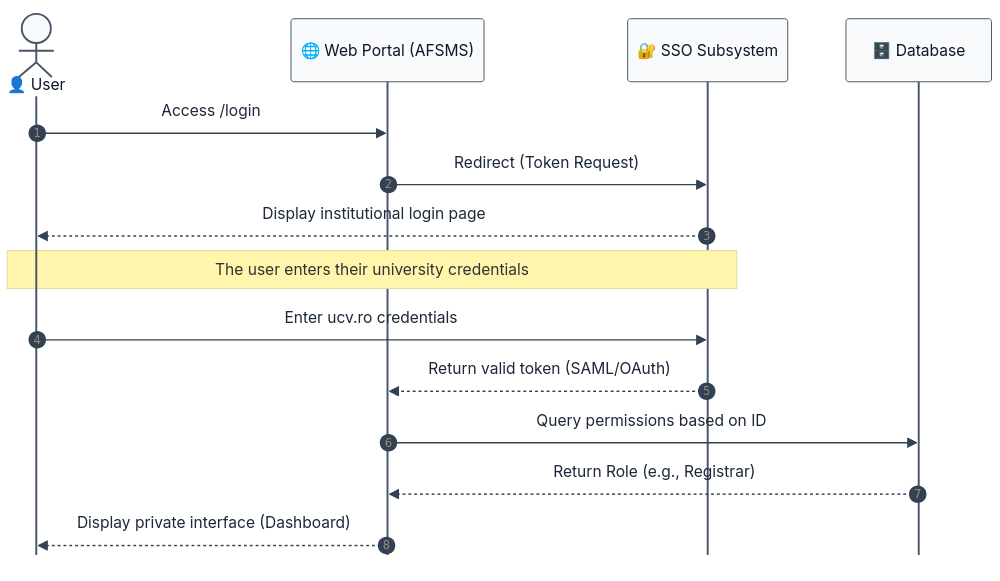
\includegraphics[width=0.9\textwidth]{2e.png}
    \caption{Web Portal and Access Management - SSO Authentication.}
    \label{fig:img2}
\end{figure}

\subsection{Academic Data Collection and Management}
\subsubsection{Description and Priority}
The system shall support the collection and management of academic data related to curricula (study plans), study formations, and enrolled students, using the web interface.

The system shall provide data extraction/import from multiple sources (databases, Excel files, text files) and shall support filters and transformations required to integrate the data into the system database.

\textbf{Priority:} High.

\subsubsection{Stimulus/Response Sequences}
\begin{table}[H]
\begin{tabularx}{\textwidth}{>{\raggedright\arraybackslash}p{6cm} >{\raggedright\arraybackslash}X}
\toprule
\textbf{Stimulus} & \textbf{Response} \\
\midrule
User opens Data Collection module. & System displays interface with selection lists for curriculum/formation/students. \\
\midrule
User selects target entity to view/edit. & System loads dataset, displays in tabular form. \\
\midrule
User imports data from external source. & System processes import, validates, makes available for integration. \\
\midrule
User configures filters/transformations. & System applies transformations, updates dataset for review. \\
\midrule
User saves integrated data. & System persists changes, makes available for reporting. \\
\midrule
User provides invalid input. & System rejects input, displays error with resolution suggestions. \\
\bottomrule
\end{tabularx}
\end{table}

\subsubsection{Functional Requirements}
\begin{itemize}
    \item \textbf{REQ-AFSMS-16:} The system shall allow collecting data corresponding to curricula (study plans), study formations, and their students.
    \item \textbf{REQ-AFSMS-17:} The system shall allow data collection and data editing through the web interface.
    \item \textbf{REQ-AFSMS-18:} The system shall provide data extraction/import capabilities from databases, Excel files, and text files.
    \item \textbf{REQ-AFSMS-19:} The system shall provide filters and data transformations required to integrate imported data into the system database.
    \item \textbf{REQ-AFSMS-20:} The system shall display managed academic data in tabular form within the web page.
    \item \textbf{REQ-AFSMS-21:} The system shall use selection lists to support easy visualization and localization of data.
    \item \textbf{REQ-AFSMS-22:} The system shall validate user-entered and imported data in the UI module and shall generate error messages for invalid inputs.
    \item \textbf{REQ-AFSMS-23:} For frequent validation errors, the system shall suggest resolution methods in the displayed error messages.
    \item \textbf{REQ-AFSMS-24:} The system shall support modifying existing academic data records, subject to the user's assigned rights.
\end{itemize}

\subsection{Reporting and Export}
\subsubsection{Description and Priority}
The system shall provide a reporting module that allows authorized users to generate academic reports based on managed data and user rights.

The reporting component shall support saving/exporting reports in multiple formats (CSV, XML, XLS, PDF) and shall generate the e-Grade Centralizer at specialization/year/form-of-education level with students in alphabetical order.

\textbf{Priority:} High.

\subsubsection{Stimulus/Response Sequences}
\begin{table}[H]
\begin{tabularx}{\textwidth}{>{\raggedright\arraybackslash}p{6cm} >{\raggedright\arraybackslash}X}
\toprule
\textbf{Stimulus} & \textbf{Response} \\
\midrule
An authenticated user opens the Reporting module. & The system displays available report types and report parameters in the web interface. \\
\midrule
The user selects the e-Grade Centralizer report and chooses specialization, year of study, and form of education. The user triggers report generation. & The system prepares the report criteria and validates parameter completeness. The system generates the report and displays it in tabular form, listing students in alphabetical order (for the e-Grade Centralizer). \\
\midrule
The user selects an export format (CSV, XML, XLS, or PDF). & The system exports the report in the selected format and provides it for download. \\
\midrule
The user attempts to generate/export a report without sufficient rights. & The system blocks the operation and displays an access-denied message. \\
\midrule
Report generation fails due to missing/invalid parameters. & The system rejects the request and displays an error message. \\
\bottomrule
\end{tabularx}
\end{table}

\subsubsection{Functional Requirements}
\begin{itemize}
    \item \textbf{REQ-AFSMS-25:} The system shall include a reporting module.
    \item \textbf{REQ-AFSMS-26:} The system shall allow authorized users to generate reports in accordance with their allocated rights.
    \item \textbf{REQ-AFSMS-27:} The system shall generate the e-Grade Centralizer at the level of specialization, year of study, and form of education.
    \item \textbf{REQ-AFSMS-28:} The system shall list students in alphabetical order within the e-Grade Centralizer report.
    \item \textbf{REQ-AFSMS-29:} The reporting component shall allow saving/exporting reports in CSV, XML, XLS, and PDF formats.
    \item \textbf{REQ-AFSMS-30:} The system shall display generated reports in tabular form in the web interface.
    \item \textbf{REQ-AFSMS-31:} If a user attempts to generate or export a report without sufficient rights, the system shall block the operation and display an access-denied message.
    \item \textbf{REQ-AFSMS-32:} If report parameters are missing or invalid, the system shall reject the report generation request and display an error message.
\end{itemize}

\begin{figure}[htbp]
    \centering
    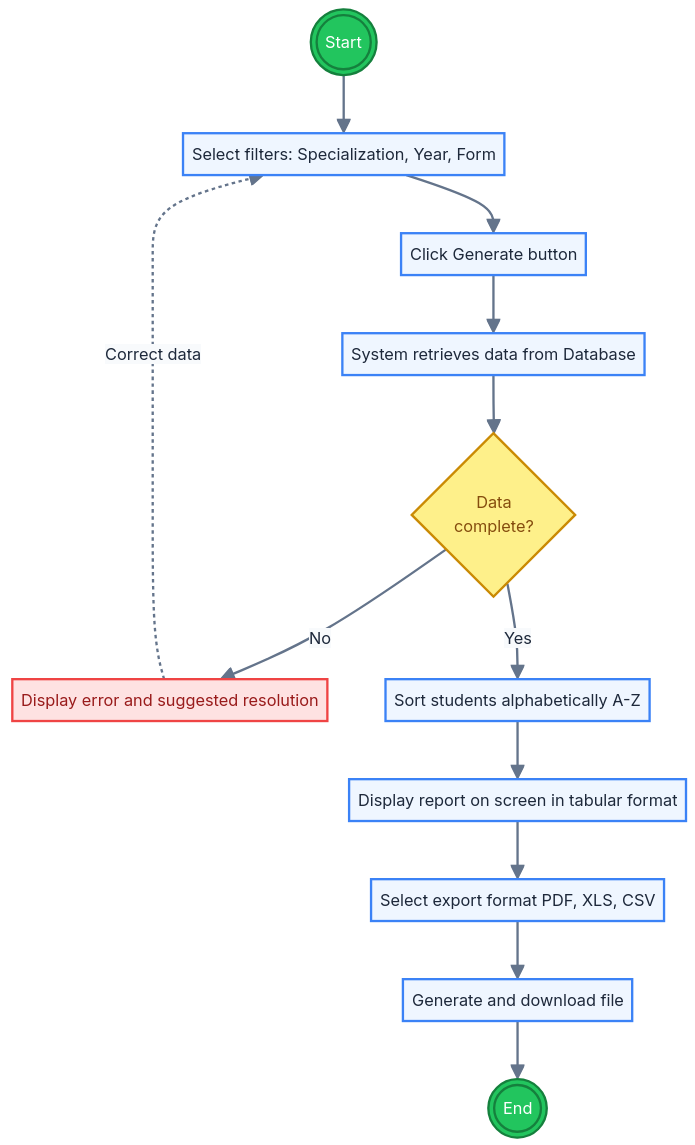
\includegraphics[width=0.9\textwidth]{3e.png}
    \caption{Reporting and Export - e-Grade Centralizer.}
    \label{fig:img3}
\end{figure}

\subsection{Document Workflow and Search}
\subsubsection{Description and Priority}
The system shall provide document workflow management for the faculty secretariat, supporting electronic circulation of documents for information, approval, or modification, as well as electronic storage and retrieval.

The system shall allow searching documents by file type, creation date, author, and document content.

\textbf{Priority:} Medium-High.

\subsubsection{Stimulus/Response Sequences}
\begin{table}[H]
\begin{tabularx}{\textwidth}{>{\raggedright\arraybackslash}p{6cm} >{\raggedright\arraybackslash}X}
\toprule
\textbf{Stimulus} & \textbf{Response} \\
\midrule
An authenticated user opens the Document Management module. & The system displays the document workspace (document list and available actions) in the web interface. \\
\midrule
The user submits/forwards a document for information, approval, or modification. & The system records the workflow action and updates the document's state and availability for retrieval. \\
\midrule
The user searches for a document by file type. & The system returns documents matching the specified file type. \\
\midrule
The user searches for a document by creation date and/or author. & The system returns documents matching the specified metadata criteria. \\
\midrule
The user searches for a document by content. & The system returns documents matching the content query. \\
\midrule
The user opens a document from search results. & The system retrieves the document and displays/downloads it according to the user's rights. \\
\midrule
The user provides invalid search criteria (e.g., malformed date). & The system rejects the search request and displays an error message. \\
\bottomrule
\end{tabularx}
\end{table}

\subsubsection{Functional Requirements}
\begin{itemize}
    \item \textbf{REQ-AFSMS-33:} The system shall support document workflow management within the faculty secretariat.
    \item \textbf{REQ-AFSMS-34:} The system shall support electronic circulation of documents for information, approval, or modification.
    \item \textbf{REQ-AFSMS-35:} The system shall support electronic storage and retrieval of documents.
    \item \textbf{REQ-AFSMS-36:} The system shall allow searching documents by file type.
    \item \textbf{REQ-AFSMS-37:} The system shall allow searching documents by creation date.
    \item \textbf{REQ-AFSMS-38:} The system shall allow searching documents by author.
    \item \textbf{REQ-AFSMS-39:} The system shall allow searching documents by document content.
    \item \textbf{REQ-AFSMS-40:} The system shall restrict document access and document workflow actions according to the user's assigned rights.
    \item \textbf{REQ-AFSMS-41:} If search input criteria is invalid, the system shall reject the search request and display an error message.
\end{itemize}

\begin{figure}[htbp]
    \centering
    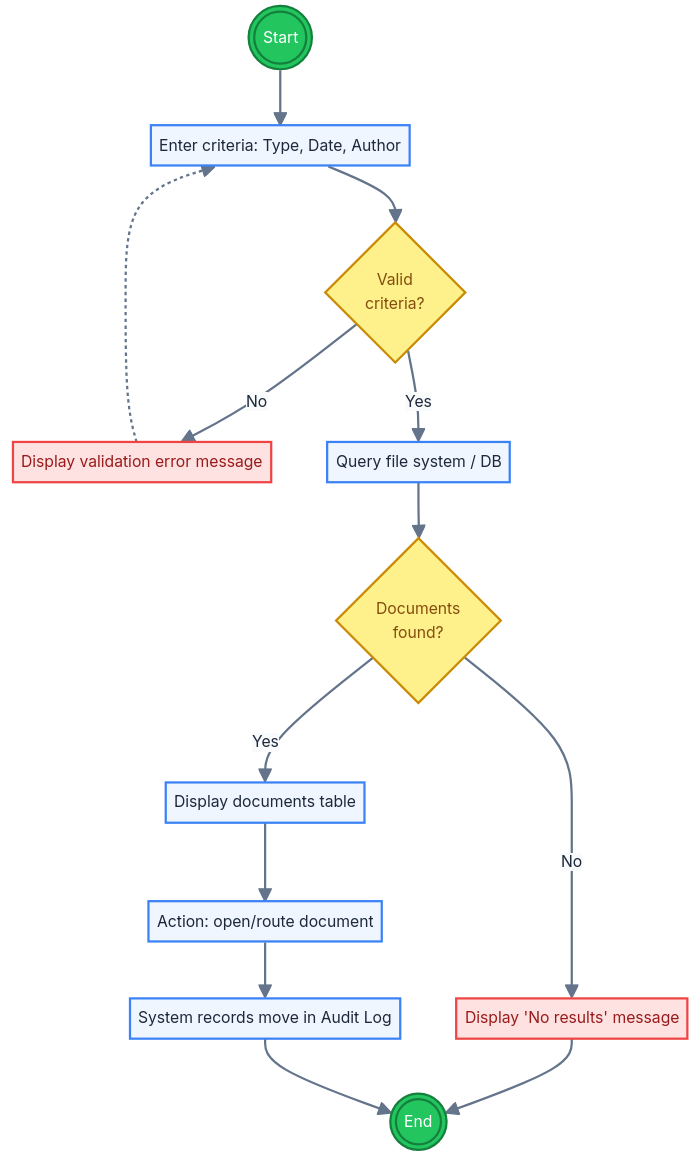
\includegraphics[width=0.9\textwidth]{4e.png}
    \caption{Document Workflow and Search - Management Interface.}
    \label{fig:img4}
\end{figure}

\subsection{User Groups and Messaging}
\subsubsection{Description and Priority}
The system shall allow defining user groups and executing operations at group level, including sending email messages to all members of a group.

The system shall support integration with Microsoft Outlook for messaging/communication use cases.

\textbf{Priority:} Medium.

\subsubsection{Stimulus/Response Sequences}
\begin{table}[H]
\begin{tabularx}{\textwidth}{>{\raggedright\arraybackslash}p{6cm} >{\raggedright\arraybackslash}X}
\toprule
\textbf{Stimulus} & \textbf{Response} \\
\midrule
An authenticated user opens the Groups module. & The system displays existing groups and the available group management actions. \\
\midrule
The user creates a new group and selects members. & The system creates the group and stores its membership. \\
\midrule
The user selects a group-level operation (e.g., ``Send email to group''). & The system prepares the operation for execution on all group members. \\
\midrule
The user sends an email message to the group. & The system sends an email message to all members of the selected group (via the supported messaging integration). \\
\midrule
The user attempts a group operation without sufficient rights. & The system blocks the operation and displays an access-denied message. \\
\bottomrule
\end{tabularx}
\end{table}

\subsubsection{Functional Requirements}
\begin{itemize}
    \item \textbf{REQ-AFSMS-42:} The system shall allow defining user groups.
    \item \textbf{REQ-AFSMS-43:} The system shall allow executing operations at group level.
    \item \textbf{REQ-AFSMS-44:} The system shall allow sending email messages to all members of a user group.
    \item \textbf{REQ-AFSMS-45:} The system shall support integration with Microsoft Outlook for messaging/communication functions.
    \item \textbf{REQ-AFSMS-46:} The system shall restrict group management and group operations according to the user's assigned rights.
\end{itemize}

\subsection{Validation and Error Handling}
\subsubsection{Description and Priority}
The system shall validate user-entered data within the user interface module and shall generate clear error messages for invalid inputs.

For frequent error cases, the system shall suggest resolution methods to help users correct input and reduce repeated mistakes.

\textbf{Priority:} High.

\subsubsection{Stimulus/Response Sequences}
\begin{table}[H]
\begin{tabularx}{\textwidth}{>{\raggedright\arraybackslash}p{3.2cm} >{\raggedright\arraybackslash}X}
\toprule
\textbf{Stimulus} & \textbf{Response} \\
\midrule
A user enters data in a web form (e.g., during data collection or report parameter selection). & The system validates the entered values in the UI module and allows the user to proceed only if the input is valid. \\
\midrule
A user submits invalid input (wrong format, missing mandatory field). & The system rejects the submission and displays an error message indicating what is invalid. \\
\midrule
A user repeatedly triggers a known frequent validation error. & The system displays the error message and suggests a resolution method. \\
\midrule
A user corrects the invalid fields and resubmits. & The system re-validates the input and, if valid, accepts it and continues the requested operation. \\
\bottomrule
\end{tabularx}
\end{table}

\subsubsection{Functional Requirements}
\begin{itemize}
    \item \textbf{REQ-AFSMS-47:} The system shall validate user-entered data within the UI module.
    \item \textbf{REQ-AFSMS-48:} If input data is invalid, the system shall reject the input and display an error message.
    \item \textbf{REQ-AFSMS-49:} For frequent validation error cases, the system shall suggest resolution methods in the displayed error messages.
    \item \textbf{REQ-AFSMS-50:} The system shall prevent saving or submitting invalid data to the database.
\end{itemize}

\subsection{Audit Logging and Data Recovery}
\subsubsection{Description and Priority}
The system shall record all executed operations and shall store activity logs containing the user who performed the action and relevant details about accessed/modified data.

The system shall provide rollback capability to return to previous data states in order to prevent and correct data collection errors; database recovery at a specified point in time and offline backup support shall be available.

\textbf{Priority:} High.

\subsubsection{Stimulus/Response Sequences}
\begin{table}[H]
\begin{tabularx}{\textwidth}{>{\raggedright\arraybackslash}p{6cm} >{\raggedright\arraybackslash}X}
\toprule
\textbf{Stimulus} & \textbf{Response} \\
\midrule
A user performs an operation (create/update/delete/import/export/report generation). & The system records the operation in the activity log, including the acting user and relevant data details. \\
\midrule
An administrator reviews system activity. & The system provides access to log records for monitoring and audit purposes (subject to rights). \\
\midrule
An administrator triggers rollback to a previous data state. & The system restores data to the selected previous state and confirms completion. \\
\midrule
A rollback operation is completed. & The system records the rollback execution as a logged activity. \\
\midrule
A recovery to a specified point in time is requested at database level. & The system/database restores data to the specified time point (point-in-time recovery), consistent with available backups/logs. \\
\midrule
Offline backup is scheduled or triggered. & The system/database produces an offline backup that can be used for recovery. \\
\bottomrule
\end{tabularx}
\end{table}

\subsubsection{Functional Requirements}
\begin{itemize}
    \item \textbf{REQ-AFSMS-51:} The system shall record all executed operations.
    \item \textbf{REQ-AFSMS-52:} For each logged activity, the system shall store the user identity that performed the action.
    \item \textbf{REQ-AFSMS-53:} For each logged activity, the system shall store relevant details about the accessed/modified data.
    \item \textbf{REQ-AFSMS-54:} The system shall provide rollback capability to return to previous data states to prevent/correct data collection errors.
    \item \textbf{REQ-AFSMS-55:} The system/database shall support recovery of data to a specified point in time.
    \item \textbf{REQ-AFSMS-56:} The system/database shall support offline backup to enable data recovery.
    \item \textbf{REQ-AFSMS-57:} The system shall restrict access to logs and rollback/recovery operations according to assigned rights.
\end{itemize}

\begin{figure}[htbp]
    \centering
    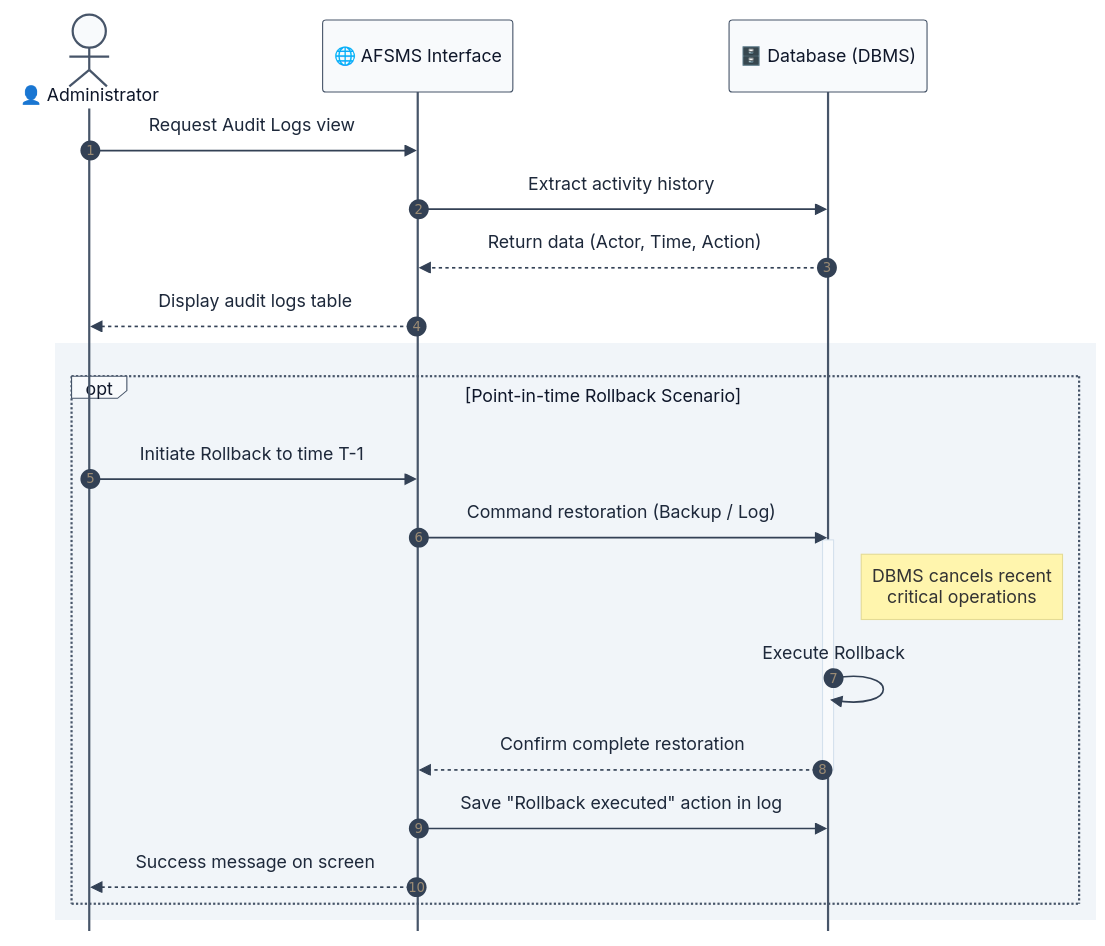
\includegraphics[width=0.9\textwidth]{5e.png}
    \caption{Audit Logging and Data Recovery - Rollback.}
    \label{fig:img5}
\end{figure}

% --- SECTION 5: OTHER NONFUNCTIONAL REQUIREMENTS ---
\section{Other Nonfunctional Requirements}

\subsection{Performance Requirements}
This subsection specifies measurable, verifiable performance constraints for AFSMS under normal and peak workload conditions, as recommended by the SRS template (quantitative statements, percentiles, and explicit workload definitions).

\textbf{NFR identifiers:}
All performance requirements are uniquely identified using the tag format NFR-AFSMS-PERF-XX to ensure traceability and testability.

\subsubsection{Capacity (Static numerical requirements)}
\begin{itemize}
    \item \textbf{NFR-AFSMS-PERF-01:} The system shall support web-based access for all user interactions without requiring special client hardware or software beyond a standard web browser.
    \item \textbf{NFR-AFSMS-PERF-02:} The database shall support managing a large volume of academic data related to students' academic status (including historical data growth).
    \item \textbf{NFR-AFSMS-PERF-03:} The system shall support concurrent user access to information in the database.
    \item \textbf{NFR-AFSMS-PERF-04:} The database management system shall support web-based administration, concurrent access, and monitoring of queries.
    \item \textbf{NFR-AFSMS-PERF-05 (TBD):} The system shall support at least TBD simultaneous authenticated users and at least TBD total stored academic records/documents, measured in the production-like environment.
\end{itemize}

\subsubsection{Response time and throughput (Dynamic numerical requirements)}
\textit{(Where feasible, dynamic targets are expressed as percentiles and tied to workload + dataset size to remain measurable.)}
\begin{itemize}
    \item \textbf{NFR-AFSMS-PERF-06 (TBD):} For interactive portal actions (open module page; load a tabular view), 95\% of requests shall complete in $\leq$ TBD seconds under normal workload.
    \item \textbf{NFR-AFSMS-PERF-07 (TBD):} For academic dataset listing using selection lists (locate and load an entity list), 95\% of requests shall complete in $\leq$ TBD seconds under normal workload and dataset size up to TBD rows.
    \item \textbf{NFR-AFSMS-PERF-08 (TBD):} Document search requests (search by file type, creation date, author, or content) shall return results in $\leq$ TBD seconds for 95\% of queries, for a repository size up to TBD documents.
    \item \textbf{NFR-AFSMS-PERF-09 (TBD):} Report generation requests (including the e-Grade Centralizer) shall complete in $\leq$ TBD seconds for 95\% of requests, for report size up to TBD students, under normal workload.
    \item \textbf{NFR-AFSMS-PERF-10 (TBD):} Exporting a generated report shall complete in $\leq$ TBD seconds for 95\% of requests for each supported format: CSV, XML, XLS, and PDF, for reports up to TBD rows.
\end{itemize}

\subsubsection{Background operations and recovery performance}
\begin{itemize}
    \item \textbf{NFR-AFSMS-PERF-11 (TBD):} Offline backup operations shall be supported and schedulable, and shall not cause user-visible downtime longer than TBD minutes during planned backup windows.
    \item \textbf{NFR-AFSMS-PERF-12 (TBD):} Point-in-time recovery and rollback operations shall be supported by the system/database and shall complete within TBD for the standard recovery scenario defined in the test plan (TBD dataset size).
\end{itemize}

\subsubsection{Performance measurement conditions (Verification)}
\begin{itemize}
    \item \textbf{NFR-AFSMS-PERF-13:} Each performance requirement shall be verified in a controlled environment and documented with: workload type (normal/peak), number of concurrent users, dataset size (rows/documents), and network conditions.
    \item \textbf{NFR-AFSMS-PERF-14:} Performance requirements shall be validated through dedicated performance tests, consistent with the project's requirement to include performance testing.
\end{itemize}

\subsection{Safety Requirements}
This section specifies requirements intended to prevent loss, corruption, or irreversible modification of critical academic data and documents, as recommended by the SRS template (define safeguards, required actions, and actions that must be prevented).

These safety requirements are derived from Tema 4 constraints related to rollback/recovery, offline backup, audit logging, data validation, and controlled access to operations.

\textbf{Safety requirement identifiers:}
Safety requirements are uniquely identified using NFR-AFSMS-SAFE-XX to support verification and traceability.

\subsubsection{Data integrity and loss prevention}
\begin{itemize}
    \item \textbf{NFR-AFSMS-SAFE-01:} The system shall record all executed operations to support auditing and incident investigation after harmful or erroneous actions.
    \item \textbf{NFR-AFSMS-SAFE-02:} The system shall provide rollback capability to return to previous data states to prevent or correct data collection errors.
    \item \textbf{NFR-AFSMS-SAFE-03:} The database subsystem shall support point-in-time recovery to a specified time.
    \item \textbf{NFR-AFSMS-SAFE-04:} The database subsystem shall support offline backup to enable recovery after failures or major incidents.
    \item \textbf{NFR-AFSMS-SAFE-05:} The system shall ensure that rollback/recovery operations are performed in a controlled manner and the completion of such operations is recorded as an audited activity.
\end{itemize}

\subsubsection{Safe input and validation safeguards}
\begin{itemize}
    \item \textbf{NFR-AFSMS-SAFE-06:} The system shall validate user-entered data in the UI module prior to accepting it for persistence to reduce the risk of harmful invalid data.
    \item \textbf{NFR-AFSMS-SAFE-07:} When validation fails, the system shall display error messages and provide suggested resolutions for frequent error cases to reduce repeated incorrect actions.
    \item \textbf{NFR-AFSMS-SAFE-08:} The system shall prevent saving invalid data into the system database.
\end{itemize}

\subsubsection{Controlled execution of critical actions}
\begin{itemize}
    \item \textbf{NFR-AFSMS-SAFE-09:} The system shall provide differentiated access to data and operations based on user roles/rights to prevent unauthorized harmful actions.
    \item \textbf{NFR-AFSMS-SAFE-10:} The system shall restrict access to logs, rollback, and recovery functions according to user rights to prevent misuse of safety-critical capabilities.
    \item \textbf{NFR-AFSMS-SAFE-11:} The system shall ensure that only authenticated users can access the private portal perspective where data modifications and report generation are performed.
\end{itemize}

\subsubsection{Safety-related operational constraints}
\begin{itemize}
    \item \textbf{NFR-AFSMS-SAFE-12:} The system shall support safe concurrent access to information (including user/group definitions and access rights) to avoid data corruption under multi-user usage.
    \item \textbf{NFR-AFSMS-SAFE-13:} The system shall log the acting user identity and relevant accessed/modified data details for each activity to enable accountability and post-incident rollback targeting.
\end{itemize}

\subsubsection{Verification (Safety)}
\begin{itemize}
    \item \textbf{NFR-AFSMS-SAFE-14:} Safety requirements related to backup, rollback, and point-in-time recovery shall be verified through dedicated recovery test scenarios (e.g., introduce a controlled data error, then demonstrate restoration to a prior consistent state).
    \item \textbf{NFR-AFSMS-SAFE-15:} Safety requirements related to input validation shall be verified through negative test cases covering invalid formats, missing mandatory fields, and frequent error patterns.
\end{itemize}

\subsection{Security Requirements}
This section defines security and privacy requirements for protecting academic data and controlling access to system functions, consistent with the SRS template guidance for security requirements (authentication, protection of data used/created, and verifiable constraints).

The requirements below align with Tema 4: a secured web portal with differentiated access by user roles, a public/private portal perspective, authentication, activity logging with user identification, and secure database access including concurrent usage controls.

\textbf{Security requirement identifiers:}
All security requirements are uniquely identified using NFR-AFSMS-SEC-XX for traceability and verification.

\subsubsection{Authentication and session access control}
\begin{itemize}
    \item \textbf{NFR-AFSMS-SEC-01:} The system shall provide a secure web interface with differentiated access based on user roles/rights.
    \item \textbf{NFR-AFSMS-SEC-02:} The web portal shall provide two perspectives: a public (unauthenticated) perspective and a private perspective accessible only to users registered in the database.
    \item \textbf{NFR-AFSMS-SEC-03:} The system shall require user authentication for all actions that modify data, generate private reports, or access private academic records.
    \item \textbf{NFR-AFSMS-SEC-04:} The authentication mechanism shall be compliant with the institution's security subsystem (i.e., a centralized security/authentication context), to support a unified account-based login.
\end{itemize}

\subsubsection{Authorization (least privilege)}
\begin{itemize}
    \item \textbf{NFR-AFSMS-SEC-05:} The system shall enforce authorization checks for each protected operation (create, update, delete, report generation, document workflow actions) based on the authenticated user's assigned rights.
    \item \textbf{NFR-AFSMS-SEC-06:} The system shall allow definition of users and user groups with different access rights, and shall enforce these rights in all relevant modules.
    \item \textbf{NFR-AFSMS-SEC-07:} Students shall only be able to access data they are permitted to view through their rights in the private portal perspective, and the system shall prevent unauthorized access to other students' records.
\end{itemize}

\subsubsection{Secure communications and transport protection}
\begin{itemize}
    \item \textbf{NFR-AFSMS-SEC-08:} The system shall use HTTPS for communication between the user's browser and the server to protect authentication and academic data in transit.
\end{itemize}

\subsubsection{Auditability and accountability}
\begin{itemize}
    \item \textbf{NFR-AFSMS-SEC-09:} The system shall log all activities and shall identify, for each logged activity, the user who performed the action and the relevant details about the accessed/modified information.
    \item \textbf{NFR-AFSMS-SEC-10:} The system shall retain sufficient audit information to support investigation of unauthorized access attempts and to support recovery/rollback targeting when needed.
\end{itemize}

\subsubsection{Privacy and regulatory constraints}
\begin{itemize}
    \item \textbf{NFR-AFSMS-SEC-11:} The system shall comply with GDPR requirements for handling personal student data and with applicable university policies for academic data retention.
    \item \textbf{NFR-AFSMS-SEC-12:} Any example data used in documentation, training materials, or UI prototypes shall be anonymized/synthetic and must not contain real student personal data.
\end{itemize}

\subsubsection{Security verification requirements}
\begin{itemize}
    \item \textbf{NFR-AFSMS-SEC-13:} Security requirements for authentication and role-based authorization shall be verified through test cases that attempt access to restricted modules/data with insufficient rights (expected result: access denied and logged).
    \item \textbf{NFR-AFSMS-SEC-14:} Audit logging requirements shall be verified by confirming that each critical action produces a log entry containing the actor identity and relevant action context.
\end{itemize}

\subsection{Software Quality Attributes}
This section specifies additional quality characteristics (beyond performance, safety, and security) that are important for stakeholders and developers, and expresses them in verifiable terms where possible.

The selected attributes reflect Tema 4 constraints (web portal, reporting/export, document search, Excel/Outlook integration, logging, backup/rollback, and support for large data volumes and concurrent access).

\subsubsection{Usability and user experience}
\begin{itemize}
    \item \textbf{NFR-AFSMS-QUAL-01:} The user interface shall be web-based and presented through a standard browser interface.
    \item \textbf{NFR-AFSMS-QUAL-02:} Academic data and report outputs displayed in the portal workspace shall use tabular presentation to support fast reading of large datasets.
    \item \textbf{NFR-AFSMS-QUAL-03:} Where applicable, the UI shall prefer selection lists (dropdowns) over free-text input to reduce data entry errors and increase speed.
    \item \textbf{NFR-AFSMS-QUAL-04:} The system shall provide clear, non-intrusive in-workspace validation error messages and shall suggest resolutions for frequent error cases (e.g., wrong import format, missing mandatory fields).
\end{itemize}

\subsubsection{Reliability and robustness}
\begin{itemize}
    \item \textbf{NFR-AFSMS-QUAL-05:} The system shall record all executed operations in an activity log to support traceability and recovery from erroneous actions.
    \item \textbf{NFR-AFSMS-QUAL-06:} The system shall support rollback to previous data states to mitigate data collection errors.
    \item \textbf{NFR-AFSMS-QUAL-07:} The database subsystem shall support offline backups and recovery to a specified point in time to restore service after failures or major incidents.
    \item \textbf{NFR-AFSMS-QUAL-08:} The system shall support concurrent access to information without causing data corruption.
\end{itemize}

\subsubsection{Maintainability and extensibility}
\begin{itemize}
    \item \textbf{NFR-AFSMS-QUAL-09:} The system architecture shall be extensible so that new software modules can be added without negative effects on the rest of the application.
    \item \textbf{NFR-AFSMS-QUAL-10 (TBD):} The project shall define and maintain module-level boundaries for core capabilities (data collection, reporting, logging) to keep the system maintainable as required modules evolve.
\end{itemize}

\subsubsection{Portability and compatibility}
\begin{itemize}
    \item \textbf{NFR-AFSMS-QUAL-11:} The system shall be platform-agnostic on the client side by relying on standard web technologies and browser access, rather than requiring local client installation.
    \item \textbf{NFR-AFSMS-QUAL-12:} The system shall coexist with Microsoft Excel and Microsoft Outlook on registrar workstations to support day-to-day workflows.
\end{itemize}

\subsubsection{Interoperability and data exchange}
\begin{itemize}
    \item \textbf{NFR-AFSMS-QUAL-13:} The reporting component shall support saving/exporting reports in standard formats including CSV, XML, XLS, and PDF.
    \item \textbf{NFR-AFSMS-QUAL-14:} The system shall support data management through extracting/importing data from multiple sources (databases, Excel files, text files) using filters and transformations required for integration into the system database.
    \item \textbf{NFR-AFSMS-QUAL-15:} The system shall support group-level operations such as sending e-mail messages to all members of a defined group (Outlook integration context).
\end{itemize}

\subsection{Business Rules}
Business rules define operational principles (who can do what, and under which conditions) that the system must enforce through role-based access and workflow constraints.
\begin{itemize}
    \item \textbf{BR-AFSMS-01:} The Web Portal shall provide a Public area accessible to any user and a Private area accessible only to users registered in the database.
    \item \textbf{BR-AFSMS-02:} Only authenticated users in the Private area may perform operations that modify stored academic data (create/update) or generate internal reports, and the specific allowed actions shall depend on assigned rights.
    \item \textbf{BR-AFSMS-03:} New users registering through the web interface shall receive an initial predefined set of rights, and these rights shall be customizable afterward to enable differentiated access.
    \item \textbf{BR-AFSMS-04:} Academic data must be displayed in the web interface in tabular form to support administrative workflows and large datasets.
    \item \textbf{BR-AFSMS-05:} Data entry and data lookup shall prioritize selection lists (dropdowns) to make data easy to locate and to reduce entry errors.
    \item \textbf{BR-AFSMS-06:} The e-Grade Centralizer (e-Centralizator) shall be produced at the level of specialization, study year, and form of education, and students shall be listed in alphabetical order.
    \item \textbf{BR-AFSMS-07:} Reports generated by the reporting component shall be exportable/savable in standard formats including CSV, XML, XLS, and PDF.
    \item \textbf{BR-AFSMS-08:} The document search function shall allow searching by file type, creation date, author, and document content (keyword).
    \item \textbf{BR-AFSMS-09:} The system shall allow defining user groups and executing group-level operations, including sending an email message to all members of a group.
    \item \textbf{BR-AFSMS-10:} All executed operations shall be recorded, and each logged activity shall include the user who performed the action plus relevant details about accessed/modified information.
    \item \textbf{BR-AFSMS-11:} The system shall support rollback/recovery to previous data states to prevent or correct data collection errors.
    \item \textbf{BR-AFSMS-12:} The database subsystem shall support offline backup and recovery to a specified point in time, and these capabilities shall be available as part of the operational rules for system maintenance.
\end{itemize}

\subsection{Coding Standards and Code Quality Rules}
The following coding standards shall be respected during system development to ensure maintainable and high-quality source code.
\begin{itemize}
    \item \textbf{CODE-01:} All source code shall follow consistent naming conventions: classes in PascalCase and variables in camelCase.
    \item \textbf{CODE-02:} Each function shall implement a single responsibility and should not exceed 50 lines of code where possible.
    \item \textbf{CODE-03:} Code duplication shall be avoided; reusable functionality shall be placed in shared modules.
    \item \textbf{CODE-04:} All public classes and methods shall include documentation comments describing their purpose and parameters.
    \item \textbf{CODE-05:} Error handling shall be implemented for all operations interacting with external systems or files.
    \item \textbf{CODE-06:} Hard-coded values (``magic numbers'') shall be avoided; constants shall be defined in configuration files or constant definitions.
    \item \textbf{CODE-07:} Source code shall be structured in logical modules corresponding to system components.
    \item \textbf{CODE-08:} All code shall be reviewed through peer code review before integration into the main branch.
    \item \textbf{CODE-09:} Static code analysis tools shall be used to detect potential bugs and code smells.
    \item \textbf{CODE-10:} Unit tests shall be implemented for core business logic components.
\end{itemize}


% --- SECTION 6: OTHER REQUIREMENTS ---
\section{Other Requirements}
This section defines additional project requirements that are essential for legal compliance, database integrity, and system extensibility.

\subsection{Database Requirements}
\begin{itemize}
    \item \textbf{Data Retention:} The system shall maintain student academic records (e-Transcripts) indefinitely to comply with educational legislation, while system audit logs may be archived after a period of 5 years.
    \item \textbf{Relational Integrity:} Any modifications to the curriculum must not retroactively alter previously validated grades stored in the e-Grade Centralizer.
\end{itemize}

\subsection{Legal and Regulatory Requirements}
\begin{itemize}
    \item \textbf{GDPR Compliance:} All processing of personally identifiable information (PII), such as student names and identification numbers, must strictly comply with EU/Romanian General Data Protection Regulation (GDPR).
    \item \textbf{Anonymization:} Any sample data used for documentation or training purposes must be synthetic and must not contain real student information.
\end{itemize}

\subsection{Internationalization and Localization}
\begin{itemize}
    \item \textbf{Language Support:} The public portal perspective shall support both Romanian and English languages to accommodate international students and mobility programs.
    \item \textbf{Character Encoding:} All system components, including PDF and Excel export modules, must use UTF-8 encoding to ensure the correct rendering of Romanian specific characters (diacritics).
\end{itemize}

% --- APPENDICES ---
\newpage
\appendix

\section{Glossary}
\begin{itemize}
    \item \textbf{AFSMS (Automated Faculty Student Management System):} The software product being specified, designed to automate the administration of student records, curricula, and document circulation within a university faculty.
    \item \textbf{e-Registrul matricol (e-Transcript):} A secure electronic document that records a student's comprehensive academic history, including all completed disciplines, associated contact hours, and earned European Credit Transfer and Accumulation System (ECTS) credits.
    \item \textbf{e-Centralizatorul de note (e-Grade Centralizer):} A standardized electronic report that aggregates student examination results within a specific academic year, organized by specialization and study formations.
    \item \textbf{Managementul fluxului de documente (Document Workflow Management):} A system capability that facilitates the electronic routing, tracking, and storage of administrative documents for information, approval, or modification purposes.
    \item \textbf{SSO (Single Sign-On):} An authentication process that allows a user to access multiple system modules or perspectives using a single set of credentials integrated with the institutional security subsystem.
    \item \textbf{Rollback:} A data integrity function that enables the database to revert to a previously verified stable state, effectively neutralizing data corruption or massive collection errors.
\end{itemize}

\section{Analysis Models}
This appendix provides the logical models that illustrate the functional requirements and data relationships of the AFSMS. These models serve as a bridge between the requirements and the system architecture.

\subsection{High-Level System Context Diagram}
The Context Diagram defines the boundary between the AFSMS and its environment, identifying the external entities that interact with the system.
\begin{itemize}
    \item \textbf{AFSMS Core System:} Processes all academic requests, report generation, and document workflows.
    \item \textbf{External Entities:}
    \begin{itemize}
        \item \textit{Registrar/Secretariat Staff:} Provide student data, curricula updates, and document routing.
        \item \textit{Teaching Staff (Professors):} Provide examination results and grades.
        \item \textit{Students:} Receive academic standings, schedules, and grade reports.
        \item \textit{University SSO Subsystem:} Provides authentication tokens for identity verification.
        \item \textit{Microsoft Ecosystem:} Facilitates the import/export of Excel files and dispatch of Outlook communications.
    \end{itemize}
\end{itemize}

\subsection{Data Flow Diagram (DFD Level 0)}
This textual description outlines the primary data transformations as they move through the system.
\begin{enumerate}
    \item \textbf{Data Collection Process:} Accepts raw data from external files (Excel, Text) and relational databases, applying transformations and filters to integrate them into the system.
    \item \textbf{Report Processing:} Transforms stored academic records (grades, ECTS, hours) into standardized formats such as the e-Grade Centralizer and e-Transcript.
    \item \textbf{Audit \& Log Generation:} For every interaction, the system generates a log entry identifying the user and the specific data modification for safety and rollback purposes.
    \item \textbf{Workflow Management:} Directs the circulation of electronic documents within the secretariat for approval or modification.
\end{enumerate}

\subsection{Entity-Relationship Model (Conceptual)}
The ER model identifies the fundamental academic data structures and their logical relationships.
\begin{itemize}
    \item \textbf{STUDENT:} Uniquely identified by personal details; enrolled in a STUDY FORMATION.
    \item \textbf{CURRICULUM (Plan de învățământ):} Defines the set of DISCIPLINES, ECTS credits, and contact hours for a specific specialization.
    \item \textbf{GRADE:} Represents the examination result linking a STUDENT to a DISCIPLINE for a specific academic year.
    \item \textbf{USER ACCOUNT:} Mapped to ROLES and PRIVILEGES, enabling differentiated access to private perspectives.
    \item \textbf{LOG ENTRY:} An append-only record linked to a USER ACCOUNT and an OPERATION.
\end{itemize}

\subsection{High-Level System States}
The AFSMS operates in two primary logical states based on user interaction and authentication status.
\begin{itemize}
    \item \textbf{Public Portal State:} The default state where any visitor can browse unauthenticated data such as curricula or public announcements.
    \item \textbf{Private Portal State:} Activated upon successful SSO Authentication. In this state, the system provides differentiated services (Data Management, Reporting, Rollback) based on the user's assigned role (Student, Professor, or Registrar).
\end{itemize}

\section{To Be Determined List}
\begin{itemize}
    \item \textbf{TBD-1 (NFR-AFSMS-PERF-005):} The exact number of simultaneous authenticated users the server must support (initially estimated based on university data center capacity).
    \item \textbf{TBD-2 (NFR-AFSMS-PERF-010-014):} The exact maximum time thresholds, in seconds, allowed for loading tabular pages and generating massive PDF and XLS reports.
    \item \textbf{TBD-3 (Section 3.4.3):} The minimum data transfer rates and exact timeout thresholds for institutional network requests.
    \item \textbf{TBD-4 (NFR-AFSMS-QUAL-021):} The exact software module boundaries to ensure an extensible architecture without negative effects on the rest of the application.
    \item \textbf{TBD-5 (Section 3.3.4):} The specific version of the external third-party library used for official PDF rendering (e.g., iText or TCPDF).
\end{itemize}

\end{document}